\documentclass[preprint,12pt]{elsarticle}

\usepackage{amsmath,amssymb}
\usepackage{graphicx}
\usepackage{booktabs}
\usepackage{longtable}
\usepackage{etoolbox}
\usepackage{array}
\usepackage{calc}
\usepackage[normalem]{ulem}
\usepackage{newunicodechar}
\usepackage{ragged2e}
\usepackage{textcomp}
\usepackage[hidelinks]{hyperref}
\pdfstringdefDisableCommands{\def\corref#1{}}
\usepackage{url}
\usepackage{float}
\biboptions{authoryear,round}
\abstracttitle{Abstract:}
\setlength{\LTcapwidth}{\textwidth}
\emergencystretch=2em
\def\real#1{#1}
\providecommand{\tightlist}{\setlength{\itemsep}{0pt}\setlength{\parskip}{0pt}}
\providecommand{\textsubscript}[1]{\ensuremath{_{\text{#1}}}}
\providecommand{\RL}[1]{#1}
\newunicodechar{±}{\ensuremath{\pm}}
\newunicodechar{β}{\ensuremath{\beta}}
\newunicodechar{‐}{-}

\makeatletter
\patchcmd{\LT@output}{\vss}{\vfil}{}{}
\patchcmd{\LT@output}{\vss}{\vfil}{}{}
\makeatother

\hypersetup{pdfauthor={},pdfsubject={},pdfkeywords={}}
\begin{document}
\begin{frontmatter}
\title{A Leakage-Controlled Benchmark and Taxonomy-Aware Multi-Context Model for Fine-Grained Fish Species Classification on OzFish}
\begin{abstract}
Reliable marine biodiversity monitoring relies, in part, on accurate
identification of fish species in underwater surveys. Automated image
analysis can reduce the tedium of manual annotation, but assessing
progress requires certain evaluation protocols that account for the
characteristics of survey data. Related observations from the same
deployment, in particular, can compromise evaluation when distributed
across training and testing sets, while overall accuracy may conceal
poor recognition of underrepresented species and differences in the
taxonomic severity of errors. To address these evaluation challenges, we
introduce a curated fine-grained fish classification benchmark built on
the existing OzFish dataset, which comprises of 76,083 fish crops across
321 species, 127 genera, and 39 families. The benchmark uses
deployment-grouped training, validation, and testing partitions, and
combines class-balanced accuracy with species-frequency and
taxonomy-aware analyses. We evaluate eight classification systems over
three random seeds using shared partitions and metrics, including a
proposed Self-Distillation with No Labels version 3 (DINOv3)-based
multi-context classifier with gated fusion and
taxonomy-aware supervision. The proposed model achieves 69.0\% macro
accuracy and 84.2\% overall accuracy, with mean predictive performance
comparable to the evaluated Multi-context Attention and Taxonomy-Aware
Network (MATANet) implementation with a much smaller
parameter count. Ablation experiments done on the proposed model show
that hierarchical supervision reduces taxonomic error severity while
still maintaining similar species-level accuracy, whereas recognition of
poorly represented species remains challenging across the evaluated
systems. This benchmark establishes a common framework for comparing
underwater fish classifiers and identifying limitations beyond aggregate
accuracy.
\end{abstract}
\begin{keyword}
Fine-grained fish classification \sep Underwater imagery \sep Benchmark dataset \sep Long-tailed distribution \sep Taxonomy-aware learning \sep Data leakage
\par\noindent\textit{INSPEC classification codes:} C1230 (Artificial intelligence); C5260B (Computer vision and image processing techniques); C5290 (Neural computing techniques); C7860 (Agriculture, forestry and fisheries computing).
\end{keyword}
\end{frontmatter}

\section{Introduction}\label{introduction}

Marine biodiversity supports ecosystem functioning and the fisheries
that we humans depend on. However, pressures such as overfishing,
pollution, and habitat degradation threaten marine ecosystems,
emphasizing the need for reliable monitoring systems to survey current
fish species composition and abundance in order to guide
preservationists and marine experts on further management decisions
\citep{ref1,ref2}.
Underwater imagery provides a means of collecting these observations,
but reviewing large volumes of footage requires considerable time and
effort, as well as an expertise in
taxonomy\citep{ref3,ref4}.
This creates a need for automated methods that can assist researchers in
identifying fish species and processing survey imagery at scale
\citep{ref1,ref5}.

Deep learning models are increasingly developed and implemented to
enable automated analysis of marine imagery, including fish detection
and species
classification\citep{ref6,ref7,ref8}.
Their performance, however, depends in part on the characteristics and
quality of the datasets used to train and evaluate
them\citep{ref9,ref10}. Underwater imagery presents a
multitude of challenging imaging conditions, such as variable
illumination, turbidity, and occlusion, which can obscure the visual
features needed to distinguish closely related species
\citep{ref8,ref9,ref11}. Additionally, species are often
unevenly represented within these datasets, producing long-tailed
distributions in which a small number of classes account for most of the
observations while many other species have relatively few examples
\citep{ref10,ref12,ref13}. This imbalance can limit
recognition performance for poorly represented species, even when
overall classification accuracy may appear high
\citep{ref14,ref15}. Evaluating performance across
different species-frequency groups is necessary to understand how
effectively a model can recognize well-represented and poorly
represented classes \citep{ref13,ref16}. The structure of the survey data
also requires attention when defining evaluation protocols
\citep{ref17,ref18}. Multiple observations within the
same deployment may contain closely related frames or stereo views
\citep{ref4,ref19}, so assigning them independently to
training and testing sets can produce overly optimistic estimates of
performance on unseen deployments \citep{ref17,ref18,ref20}.

These challenges highlight the necessity for benchmarks that evaluate
recognition performance across unevenly represented species while also
accounting for the structure of underwater survey data
\citep{ref10,ref13,ref21}. To support systematic evaluation
under these conditions, we introduce a fine-grained fish classification
benchmark built on the existing OzFish dataset
\citep{ref22}. The curated benchmark contains
76,083 fish crops that span 321 species, 127 genera, and 39 families. We
partition the data at the Baited Remote Underwater Video Station (BRUVS)
deployment level \citep{ref4}, keeping
observations from the same deployment within a single partition,
preventing overlap between training, validation, and testing sets
\citep{ref17,ref18}. The evaluation combines overall
and class-balanced accuracy with species-frequency analyses
\citep{ref16} and taxonomy-aware metrics
\citep{ref23,ref24}, providing complementary
perspectives on model performance.

We evaluate eight different classification models using this benchmark,
spanning convolutional networks, supervised vision transformers, a
self-supervised representation baseline, and context-aware approaches.
These include our proposed DINOv3-based model
\citep{ref25} that draws inspiration from
MATANet's multi-context architecture
\citep{ref26}, combining target appearance with
surrounding visual information through gated fusion. The model,
hereafter referred to as Bio-TAC (Biological Taxonomy-Aware Classification), also incorporates taxonomy-aware
supervision by deriving genus and family probabilities from its species
predictions \citep{ref24,ref26}. All models are evaluated using
shared data partitions and a common set of classification and
taxonomy-aware metrics, with results reported across three random seeds.
Model parameter count was also compared between the different models
alongside predictive performance. Additional ablation experiments on
Bio-TAC investigate the effects of backbone adaptation, contextual
inputs, hierarchical supervision, and long-tail training strategies.

\section{Related Work}\label{related-work}

This section reviews prior work on underwater image datasets for fish
recognition, fine-grained recognition and visual representations,
environmental context in marine recognition, taxonomy-aware and
long-tailed learning objectives, and evaluation protocols for ecological
data. It closes by summarizing the gaps that motivate the benchmark and
the model developed in this paper.

\subsection{Underwater Image Datasets for Fish
Recognition}\label{underwater-image-datasets-for-fish-recognition}

Several public datasets have been developed for automated fish
recognition, and they differ considerably in imaging conditions, label
granularity, and intended task. Fish4Knowledge
\citep{ref3} was among the first large
collections of in-situ underwater video, recorded by fixed cameras on
coral reefs in Taiwan, and the LifeCLEF fish tasks
\citep{ref27} used this footage to organize fish
identification as a shared evaluation challenge. WildFish
\citep{ref28} and its extension WildFish++
\citep{ref29} are much broader taxonomically,
reaching 2,348 categories, but both are built from web imagery whose
appearance differs substantially from survey footage. DeepFish
\citep{ref9} contains in-situ video from
Australian habitats, although its classification task separates fish
from background rather than identifying species. FathomNet
\citep{ref30} has become an important open
resource for deep-sea imagery, providing taxonomically labelled
detections across a wide range of midwater and benthic taxa, and a
curated subset of it was released for the FathomNet 2025 fine-grained
recognition challenge at the CVPR 2025 FGVC12 workshop
\citep{ref30}. FishNet
\citep{ref10} is larger still and pairs species
labels with functional trait annotations. Broader overviews of
underwater image datasets and fish recognition methods are given by
\citet{ref5} and \citet{ref6} .

OzFish \citep{ref22} is the dataset used in this
work. It was produced under the Australian Research Data Commons Data
Discoveries programme from more than three thousand historical BRUVS
videos. Its full composition is reported in Section~\ref{dataset-source-and-collection}, and its
position relative to the other resources reviewed here is summarised in
Table~\ref{tab:public-datasets}. The annotations were made by fish ecologists following the
marine sampling field manual for benthic stereo-BRUVS
\citep{ref4}, so the dataset combines
survey-grade imagery with unusually deep and reliable taxonomic labels.
So far, however, OzFish has been used mainly for detection and
morphometry, for example in YOLO-Fish
\citep{ref7} and in the semi-automated length
measurement model of Marrable et
al.\citep{ref19}. No standard classification
split has been released for the dataset, so studies that classify OzFish
species adopt their own filtering thresholds and partitions, and their
results are neither comparable nor reproducible. These ad hoc partitions
also ignore the survey structure of the imagery, in which many crops
originate from the same deployment, so the reported accuracies may be
inflated by data leakage \citep{ref17,ref20}. This work addresses both problems
by building a curated, leakage-controlled fine-grained classification
benchmark on OzFish and releasing it with a deployment-grouped split.

Table~\ref{tab:public-datasets} compares the main public datasets for fish and marine species
recognition with the benchmark proposed in this work. Counts are
reported as provided by the original authors and may refer to images,
cropped detections, or regions of interest (ROIs). The final column
indicates whether each dataset is released with a split that keeps
images from the same survey unit, site, or deployment within a single
fold. As the final rows show, no earlier resource combines the taxonomic
depth, survey-grade imagery, and released group-aware split that a
rigorous fine-grained benchmark requires.

\footnotesize\setlength{\tabcolsep}{3pt}
\begin{longtable}[]{@{}
  >{\raggedright\arraybackslash}p{(\columnwidth - 10\tabcolsep) * \real{0.2036}}
  >{\raggedright\arraybackslash}p{(\columnwidth - 10\tabcolsep) * \real{0.1327}}
  >{\raggedright\arraybackslash}p{(\columnwidth - 10\tabcolsep) * \real{0.0980}}
  >{\raggedright\arraybackslash}p{(\columnwidth - 10\tabcolsep) * \real{0.1444}}
  >{\raggedright\arraybackslash}p{(\columnwidth - 10\tabcolsep) * \real{0.2342}}
  >{\raggedright\arraybackslash}p{(\columnwidth - 10\tabcolsep) * \real{0.1872}}@{}}
\caption{Public datasets for fish and marine species recognition.}\\
\toprule\noalign{}
\begin{minipage}[b]{\linewidth}\raggedright
Dataset
\end{minipage} & \begin{minipage}[b]{\linewidth}\raggedright
Images / crops
\end{minipage} & \begin{minipage}[b]{\linewidth}\raggedright
Species
\end{minipage} & \begin{minipage}[b]{\linewidth}\raggedright
Taxonomic levels
\end{minipage} & \begin{minipage}[b]{\linewidth}\raggedright
Imagery source
\end{minipage} & \begin{minipage}[b]{\linewidth}\raggedright
Grouped split released
\end{minipage} \\
\midrule\noalign{}
\endhead
\bottomrule\noalign{}
\endlastfoot
\label{tab:public-datasets}Fish4Knowledge (Boom et al., 2014) & 27,370 & 23 & Species & Fixed reef
cameras, Taiwan & No \\
LifeCLEF2015-Fish (Joly et al., 2015) & 9,160 ROIs & 15 & Species, order
& Fixed reef cameras, Taiwan & No \\
WildFish (Zhuang et al., 2018) & 54,459 & 1,000 & Species & Web imagery
& No \\
WildFish++ (Zhuang et al., 2020) & 103,034 & 2,348 & Species & Web
imagery & No \\
DeepFish (Saleh et al., 2020) & \textasciitilde40,000 & n/a & Fish vs.
background & In-situ video, Australia & No \\
FathomNet2025 (Barnard et al., 2025) & 23,700 ROIs & 79 taxa & Mixed
ranks & ROV and AUV, deep sea & No; test set withheld \\
FishNet (Khan et al., 2023) & 94,532 & 17,357 & Class to species &
Aggregated databases & No; random 80/20 \\
OzFish (AIMS et al., 2019) & \textasciitilde80,000 crops & 507 & Family,
genus, species & Stereo-BRUVS, Australia & No \\
This work (OzFish benchmark) & 76,083 crops & 321 & Family, genus,
species & Stereo-BRUVS, Australia & Yes; deployment-grouped \\
\end{longtable}
\normalsize\setlength{\tabcolsep}{6pt}

\subsection{Fine-Grained Recognition and Visual
Representations}\label{fine-grained-recognition-and-visual-representations}

Fine-grained visual classification concerns categories that are visually
similar to one another, as in the bird dataset CUB-200-2011
\citep{ref31} and the multi-taxon iNaturalist
dataset \citep{ref12}. In this setting the
differences between classes are small and spatially localised, while
variation within a class from pose, illumination, and background is
large \citep{ref32}. Early deep learning
approaches localised discriminative parts or modelled higher-order
feature interactions \citep{ref33,ref34,ref35}. Later work built on vision
transformers, from the original ViT \citep{ref36}
to TransFG \citep{ref37}, which selects
discriminative tokens, and hierarchical variants such as Swin
\citep{ref38}. Convolutional networks remain
competitive, from ResNet \citep{ref39} through
EfficientNetV2 \citep{ref40} to ConvNeXt
\citep{ref41} . Several of these architectures
have been applied to fish recognition, including MSDBN
\citep{ref42}, SwinFishNet
\citep{ref43}, ConvFishNet
\citep{ref44}, and the transformer study of \citet{ref45}. All of these models
operate on the cropped fish alone, and each is evaluated on a
differently constructed dataset, which makes their results hard to
compare.

A parallel line of work has changed how the underlying representations
are learned. DINO \citep{ref46} showed that
self-distillation without labels produces transformer features with
strong object-centric structure. DINOv2
\citep{ref47} scaled this approach into
general-purpose features that transfer well without fine-tuning, and
DINOv3 \citep{ref25} scaled it further,
introducing Gram anchoring to keep dense patch features from degrading
over long training schedules. The quality of these patch features
matters for context modelling, because any method that attends over
patch tokens depends on the tokens staying spatially sharp.
Language-aligned models such as CLIP
\citep{ref48} and BioCLIP
\citep{ref49}, the latter trained on a
taxonomically structured corpus, offer a complementary route. Freezing
such a backbone and training a lightweight head on top of it is
attractive in ecological applications, where labelled data are limited
relative to the capacity of a large transformer
\citep{ref50,ref51}.

Underwater imagery introduces degradations that these benchmarks do not
contain, including wavelength-dependent color attenuation, turbidity and
backscatter, marine snow, uneven illumination, motion blur, and frequent
occlusion \citep{ref8,ref11,ref52}. In BRUVS footage a fish often
occupies only a small fraction of a high-resolution frame, so the
resolution actually available for distinguishing species is far below
the nominal image size \citep{ref4,ref9}. Despite these challenges, applied
fish classification has been slow to adopt self-supervised backbones,
and end-to-end fine-tuning of ImageNet-pretrained networks remains the
norm \citep{ref6,ref51}. How much adaptation such a
backbone needs on BRUVS imagery is also unsettled. Frozen features and
full fine-tuning are usually treated as alternatives, while the
intermediate option of unfreezing only the last few transformer blocks
is rarely reported, so the point at which further adaptation stops
repaying its cost is unknown for this domain
\citep{ref51}.

\subsection{Environmental Context in Marine
Recognition}\label{environmental-context-in-marine-recognition}

Contextual information has long been known to support object recognition
in computer vision\citep{ref53,ref54,ref55,ref56}. The effect is stronger in ecology,
where habitat associations and co-occurrence patterns are part of how an
expert identifies an ambiguous specimen. The same signal can also cause
failures. \citet{ref18} showed on
camera-trap data that models learn to rely on backgrounds and locations,
and that accuracy drops sharply at sites not seen during training. Their
later Context R-CNN \citep{ref57} instead
supplies context as an explicit input rather than letting the model
absorb it implicitly. Within marine imagery, the closest work to the
model proposed in this paper is MATANet
\citep{ref26}. MATANet introduces a Multi-Context
Environmental Attention Module (MCEAM), which applies cross-attention
between the ROI representation and crops of the surrounding scene at 3×,
5×, and full-image scales, together with a Hierarchical
Separation-Induced Learning Module (HSLM) that attaches an auxiliary
classifier to each taxonomic level. In its ablation study on
FathomNet2025\citep{ref30}, hierarchical distance
improved from 2.24 with a single context stream to 1.90 with three
streams, and to 1.77 once HSLM was added. Its strongest configuration
reached 1.45 on the private challenge leaderboard, against 1.68 for the
next-best published entry \citep{ref26}. Other
entries to the same challenge also reported gains from combining
full-image context with taxonomy-aware losses
\citep{ref30}, which suggests the effect is not
specific to one architecture.

The model evaluated in this paper adopts the MCEAM formulation and
differs from MATANet \citep{ref26} in three
respects, described in Section~\ref{proposed-method}. It is built on a substantially smaller
backbone, hierarchical supervision is applied by marginalising a single
species distribution instead of through per-level auxiliary classifiers,
and evaluation is carried out on the proposed benchmark rather than on a
curated challenge set. The last difference matters because existing
context-aware results come from datasets whose partitions do not control
for the survey unit an image came from, which leaves open how much of
the reported gain is ecological evidence and how much is a
site-identifying shortcut \citep{ref17,ref18,ref58} . Capacity is a second confound.
Where context is added to a backbone that is fine-tuned end to end, any
improvement reflects both the contextual pathway and the extra trainable
parameters introduced alongside it. The ablations in Section~\ref{results-and-discussion} therefore
evaluate the contextual pathway under a fixed frozen encoder, separating
its effect from changes in backbone adaptation.

\subsection{Taxonomy-Aware and Long-Tailed Learning
Objectives}\label{taxonomy-aware-and-long-tailed-learning-objectives}

Biological taxonomy provides structure that a flat classifier ignores.
Under standard cross-entropy, confusing two species of the same genus
costs exactly as much as confusing two species from different families.
\citet{ref23} divide methods
that exploit this structure into local and global approaches. Local
methods attach a classifier to each taxonomic level and train them
jointly, as in the conditional softmax of
YOLO9000\citep{ref59}, the per-level design of
MATANet \citep{ref26}, and FishAI
\citep{ref60} , which classifies marine fish at
five taxonomic ranks and reports accuracy falling from 0.975 at class
level to 0.626 at species level. Global methods impose the hierarchy
through the loss or the label space while keeping a single output layer,
as in \citet{ref61}, the hierarchical
cross-entropy of \citet{ref24},
\citet{ref32}, and the hierarchical
multi-label contrastive method of \citet{ref62}.

Local methods are simple to implement, but they do not model
parent-child relations explicitly, and nothing forces the genus
classifier to predict a genus that contains the species chosen by the
species classifier\citep{ref23}. Marginalising a
single species distribution removes this inconsistency by construction,
at the cost of placing the full distributional burden on the species
head. This trade-off has not been examined closely against level-wise
supervision in the marine setting. Evaluation has developed along
similar lines, and lowest-common-ancestor metrics such as hierarchical
distance now credit predictions that miss the species but recover the
genus or family \citep{ref24,ref30,ref61}.

Survey data are also long-tailed, exhibiting the skewed
species-abundance distributions typical of ecological sampling, in which
a few abundant species dominate the record while most are observed only
rarely \citep{ref12,ref15}. The usual response is reweighting,
through focal loss \citep{ref63}, class-balanced
weighting by effective sample number
\citep{ref14}, or margin-based losses such as
LDAM \citep{ref64}. \citet{ref65} showed that decoupling
representation learning from classifier rebalancing often outperforms
rebalancing both jointly, and \citet{ref16} addressed the open long-tailed
setting directly. Resampling is the main alternative
\citep{ref15}, although class-balanced samplers
change both the exposure of each class and the number of optimisation
steps per epoch, an interaction that is easy to overlook under a fixed
epoch budget.

It is not yet clear which of these strategies transfer to marine data.
On FishNet, class-balanced reweighting improved rare-class accuracy
substantially, focal loss reduced it, and combining the two performed
worse than class-balancing alone \citep{ref10}.
This is a single result on a single dataset, but it indicates that
long-tail methods validated on terrestrial benchmarks should be
re-tested rather than assumed to work here. In applied fish
classification the tail is more often removed than addressed
\citep{ref6,ref8}.
Species below an occurrence threshold are discarded and results are
reported as overall accuracy, which is dominated by the abundant
classes, even though rare species are often those of greatest
conservation interest \citep{ref66}.

\subsection{Evaluation Protocols and Data
Leakage}\label{evaluation-protocols-and-data-leakage}

The reliability of a benchmark depends on how its data are partitioned.
\citet{ref17} argue that when data
carry spatial, temporal, hierarchical, or phylogenetic structure, random
cross-validation seriously underestimates predictive error, and they
recommend block cross-validation, in which the data are divided
strategically rather than at random, wherever such dependence exists.
\citet{ref20} document how
widespread the resulting leakage has become, identifying affected
results in at least 294 papers across seventeen disciplines. Underwater
survey video is a particularly difficult case. Frames from a single
BRUVS deployment can show the same individual repeatedly, consecutive
frames of the same animal, paired views from a stereo rig, and a
substrate, lighting profile, and turbidity level that barely change
\citep{ref4,ref19}. A partition drawn at the level of
individual crops therefore places near-duplicates on both sides of the
train and test boundary, and a model can score well simply by
recognising the deployment rather than the species
\citep{ref18,ref58}. The concern is even greater for a
model that is deliberately given wide-field context, because the
background is exactly the signal that identifies a deployment
\citep{ref18,ref58}. Controlling for the survey unit is
therefore a precondition for interpreting any claim that context
improves recognition.

Grouped partitioning at the level of sites or sessions is established
practice in the camera-trap literature
\citep{ref18} and follows directly from \citet{ref17}, and marine computer vision
has started to adopt it. The Caltech Fish Counting dataset
\citep{ref21} draws its training and test data
from separate sonar camera deployments, so that generalisation is
measured at unseen locations, and ReefNet
\citep{ref13} pairs a conventional within-source
split with a cross-source benchmark that withholds entire annotation
sources. Fine-grained fish classification has not followed this
practice. Random partitioning is still used even in flagship resources,
with FishNet adopting a random 80/20 division of its images
\citep{ref10}, and split definitions frequently
remain unreleased, as the final column of Table~\ref{tab:public-datasets} shows.

\subsection{Summary of Research
Gaps}\label{summary-of-research-gaps}

The review above identifies four gaps that motivate this work. First,
OzFish offers the taxonomic depth and survey provenance that a rigorous
fine-grained benchmark requires, but no released, leakage-controlled
classification split exists for it, so results reported on it are not
comparable. Second, no study has compared convolutional networks,
supervised transformers, self-supervised features under varying degrees
of backbone adaptation, and a marine-specific context-aware model on the
same underwater data under identical conditions. Third, the evidence
that environmental context helps has come from datasets that do not
control for the survey unit and from fully fine-tuned backbones, so the
effect of context has not been separated from shortcut learning or from
added model capacity. Fourth, taxonomy-aware supervision and long-tail
treatment are usually studied separately, the prevailing hierarchical
designs rely on per-level classifiers whose predictions need not agree
across levels, and the long-tail methods most commonly applied have not
been validated on marine imagery. This paper addresses these gaps by
releasing a deployment-grouped OzFish classification benchmark,
evaluating a panel of baselines on it under a common protocol, and
proposing a taxonomy-aware multi-context classifier that enforces
hierarchical consistency by marginalisation and achieves mean
performance comparable to a much larger context-aware model at a
fraction of its backbone size.

\section{Dataset Specification}\label{dataset-specification}

This section explains the construction of the OzFish classification
benchmark used during this study. It details the source dataset,
benchmark construction and filtering procedures, deployment-level
splitting strategy, and resulting taxonomic and class distribution.

\subsection{\texorpdfstring{Dataset Source and Collection
}{Dataset Source and Collection }}\label{dataset-source-and-collection}

OzFish is a publicly available dataset provided by the Australian
Institute of Marine Science (AIMS)\citep{ref22}.
The dataset contains around 80,000 fish crop images, 45,000 bounding box
annotations, and capturing 507 species belonging to 200 genera and 70
families. Each sample in the dataset contains a hierarchical annotation,
which contains which family, genus, and species the fish belongs to.

Given that the dataset was collected using Baited Remote Underwater
Video Stations (BRUVS) \citep{ref4}, makes the
captured underwater imagery include challenging conditions, such as
turbidity, motion blur, occlusions, cluttered backgrounds, etc
\citep{ref6,ref9}.
Rather than laboratory conditions, since OzFish have these
characteristics makes it a suitable benchmarking for fine-grained fish
classification in realistic marine environments.

\subsection{\texorpdfstring{Dataset Curation
}{Dataset Curation }}\label{dataset-curation}

Several requirements need to be met in a dataset for it to be suitable
for the benchmarking of fine-grained fish classification models. First,
it must have a hierarchical taxonomic label (family, genus, and species)
in order to help taxonomy-aware learning
\citep{ref23,ref24}. Second, the dataset should be
large enough to train transformer models, since transform-based models
usually benefit from massive training datasets
\citep{ref36,ref45}. Finally, the dataset images should
display realistic underwater conditions, such as motion blur, varying
light brightness, occlusions, marine snow, and other environmental
conditions, to make sure it is actually usable in real world scenarios
\citep{ref8,ref9}.

Ozfish dataset satisfies these requirements by including hierarchical
taxonomic labels, a large number of annotated underwater images, and
data captured using BRUVS under realistic underwater conditions.
Therefore, it is well suited for benchmarking taxonomy-aware
fine-grained classification and modern transformer-based architectures.

To create a standard and reproducible benchmark, the original OzFish
dataset was curated by applying label cleaning and filtering species.

\subsubsection{\texorpdfstring{Label Cleaning
}{Label Cleaning }}\label{label-cleaning}

Prior to benchmark construction, the original OzFish metadata underwent
a label cleaning process to ensure consistent and reliable taxonomic
annotations. Since the benchmark aims to support taxonomy-aware
fine-grained classification, inconsistencies in species naming or
ambiguous labels could artificially increase the number of classes and
negatively affect both model training and evaluation.

First, species labels were represented using their complete scientific
binomial names, consisting of both the genus and species identifiers,
rather than using the species epithet alone. This prevents different
biological species from being merged into the same class when identical
species epithets exist across different genera. In addition, known
taxonomic spelling inconsistencies were standardized to a canonical
representation to avoid duplicate class definitions caused by formatting
or naming variations.

Furthermore, placeholder labels that do not correspond to valid species
annotations were removed from the benchmark. Such labels provide
ambiguous supervision and may introduce incorrect class information
during training. By eliminating these samples and standardizing the
remaining taxonomic annotations, the resulting benchmark provides a
consistent and biologically meaningful label space suitable for
taxonomy-aware learning.

\subsubsection{\texorpdfstring{Species Filtering
}{Species Filtering }}\label{species-filtering}

Even though the OzFish dataset contains a large number of unique
species, 507 unique species to be exact, many of those species do not
have enough samples for the model to learn about the species, since it
cannot evaluate them fairly, having that the metrics would be unstable
and unusable in this case, which leads to a poor train, validation, and
testing representation. Therefore, inclusion rules had to be set in
order to benchmark the OzFish dataset fairly and correctly. First, a
species is included if it has at least 20 crops in the dataset, which is
the minimum number of crops which provides sufficient samples for
training and feasible dataset partitioning. Afterwards, the species
should appear in at least three deployments, which will be explained in
detail in Section~\ref{dataset-splits}.

Hence, Table~\ref{tab:dataset-comparison} shows what are the final numbers of crops, species,
genera, families, and deployments that were included in the final
benchmark compared to the original OzFish.

\footnotesize\setlength{\tabcolsep}{3pt}
\begin{longtable}[]{@{}
  >{\raggedright\arraybackslash}p{(\columnwidth - 4\tabcolsep) * \real{0.3265}}
  >{\raggedright\arraybackslash}p{(\columnwidth - 4\tabcolsep) * \real{0.3367}}
  >{\raggedright\arraybackslash}p{(\columnwidth - 4\tabcolsep) * \real{0.3367}}@{}}
\caption{Comparison of the original OzFish dataset and the final benchmark.}\label{tab:dataset-comparison}\\
\toprule\noalign{}
\begin{minipage}[b]{\linewidth}\raggedright
Metric
\end{minipage} & \begin{minipage}[b]{\linewidth}\raggedright
Original Dataset
\end{minipage} & \begin{minipage}[b]{\linewidth}\raggedright
Final Benchmark
\end{minipage} \\
\midrule\noalign{}
\endhead
\bottomrule\noalign{}
\endlastfoot
Crops & \textasciitilde80,000 & 76,083 \\
Species & 507 & 321 \\
Genera & 200 & 127 \\
Families & 70 & 39 \\
Deployments & 1,589 & 1,548 \\
\end{longtable}
\normalsize\setlength{\tabcolsep}{6pt}

\subsection{\texorpdfstring{Dataset Splits
}{Dataset Splits }}\label{dataset-splits}

The chosen samples are partitioned based on their original BRUVS
deployments in order to ensure that the benchmark offers reliable
evaluation of model generalization. The subsections describe the
motivation for deployment-level grouping, the stratification procedure,
and leakage safe splitting.

\subsubsection{Deployment-Level Splitting
Strategy}\label{deployment-level-splitting-strategy}

An important part of creating a trustworthy image classification
benchmark is making sure that the training, validation, and testing
partitions remain statistically independent. Unlike conventional image
datasets, since OzFish is collected using BRUVS
\citep{ref4,ref22}, performing a random crop level
split allows highly similar images, or even the same individual fish, to
appear at the same time in both the training and testing sets.
Consequently, it introduces data leakage, which leads to overly positive
performance estimates that do not accurately show the model's ability to
generalize \citep{ref17,ref18,ref20}.

Therefore, the proposed benchmark performs dataset partitioning at the
single indivisible unit to eliminate this problem
\citep{ref17}. In order to ensure that every
image originates from the same deployment is appointed only to either
the training, validation, or testing partition, each BRUVS deployment is
treated as a single indivisible unit. Using this method, it guarantees
that stereo images pairs captured during the same deployment
\citep{ref4,ref19}
remain within the same split, avoiding leakage between partitions.

\subsubsection{Grouped Stratified
Partitioning}\label{grouped-stratified-partitioning}

While maintaining deployment integrity, the benchmark also seeks to
preserve representative species distributions across the three
partitions. Therefore, a grouped stratified splitting strategy was
adopted, targeting an approximate 70\%/15\%/15\% distribution for the
training, validation, and testing sets, respectively. Since deployments
contain varying numbers of images and species compositions, the final
proportions cannot always match the target ratios exactly. Instead, the
splitting algorithm prioritizes maintaining deployment integrity while
distributing species as evenly as possible among the three partitions.

The resulting benchmark statistics are presented in Table~\ref{tab:split-statistics}, where the
final dataset consists of 50,513 training crops, 12,458 validation
crops, and 13,112 testing crops. These correspond to approximately
66.39\%, 16.37\%, and 17.23\% of the complete benchmark, respectively.
Despite the constraints imposed by grouped splitting, all 321 species
are represented within the training partition, while the validation and
testing partitions preserve the vast majority of the taxonomic
diversity.

\footnotesize\setlength{\tabcolsep}{3pt}
\begin{longtable}[]{@{}
  >{\raggedright\arraybackslash}p{(\columnwidth - 12\tabcolsep) * \real{0.1150}}
  >{\raggedright\arraybackslash}p{(\columnwidth - 12\tabcolsep) * \real{0.1251}}
  >{\raggedright\arraybackslash}p{(\columnwidth - 12\tabcolsep) * \real{0.1540}}
  >{\raggedright\arraybackslash}p{(\columnwidth - 12\tabcolsep) * \real{0.1444}}
  >{\raggedright\arraybackslash}p{(\columnwidth - 12\tabcolsep) * \real{0.1444}}
  >{\raggedright\arraybackslash}p{(\columnwidth - 12\tabcolsep) * \real{0.1348}}
  >{\raggedright\arraybackslash}p{(\columnwidth - 12\tabcolsep) * \real{0.1824}}@{}}
\caption{Dataset Split Statistics}\label{tab:split-statistics}\\
\toprule\noalign{}
\begin{minipage}[b]{\linewidth}\raggedright
Split
\end{minipage} & \begin{minipage}[b]{\linewidth}\raggedright
Crops
\end{minipage} & \begin{minipage}[b]{\linewidth}\raggedright
Percentage
\end{minipage} & \begin{minipage}[b]{\linewidth}\raggedright
Species
\end{minipage} & \begin{minipage}[b]{\linewidth}\raggedright
Genera
\end{minipage} & \begin{minipage}[b]{\linewidth}\raggedright
Families
\end{minipage} & \begin{minipage}[b]{\linewidth}\raggedright
Deployments
\end{minipage} \\
\midrule\noalign{}
\endhead
\bottomrule\noalign{}
\endlastfoot
Train & 50,513 & 66.39\% & 321 & 127 & 39 & 1,054 \\
Val & 12,458 & 16.37\% & 313 & 125 & 38 & 264 \\
Test & 13,112 & 17.23\% & 311 & 123 & 39 & 230 \\
\end{longtable}
\normalsize\setlength{\tabcolsep}{6pt}

The deployment statistics are summarized in Table~\ref{tab:deployment-statistics}. The benchmark
contains 1,548 unique BRUVS deployments, with an average of 49.15 image
crops per deployment and a median of 16 crops. The large variation in
deployment sizes, ranging from a single crop to 630 crops, further
demonstrates why deployment-level grouping is necessary, as random
image-level partitioning would likely distribute highly correlated
samples across different dataset splits.

\begingroup
\footnotesize\setlength{\tabcolsep}{3pt}
\setlength{\LTpre}{0pt}
\setlength{\LTpost}{2pt}
\renewcommand{\arraystretch}{0.70}
\begin{longtable}[]{@{}
  >{\raggedright\arraybackslash}p{(\columnwidth - 2\tabcolsep) * \real{0.5000}}
  >{\raggedright\arraybackslash}p{(\columnwidth - 2\tabcolsep) * \real{0.5000}}@{}}
\caption{Deployment Statistics}\\
\toprule\noalign{}
\begin{minipage}[b]{\linewidth}\raggedright
Statistics
\end{minipage} & \begin{minipage}[b]{\linewidth}\raggedright
Value
\end{minipage} \\
\midrule\noalign{}
\endhead
\bottomrule\noalign{}
\endlastfoot
Total Deployments & 1548 \\
Mean Crops per Deployment & 49.15 \\
Median Crops per Deployment & 16 \\
Min Crops per Deployment & 1 \\
Max Crops per Deployment & 630 \\
\end{longtable}
\makeatletter\edef\@currentlabel{\thetable}\def\@currentlabelname{Deployment Statistics}\makeatother
\label{tab:deployment-statistics}
\endgroup
\normalsize\setlength{\tabcolsep}{6pt}

\subsubsection{Leakage Verification}\label{leakage-verification}

For the purpose of ensuring the integrity of the benchmark, following
the partition generation an automated verification procedure was
performed. The verification confirmed that no deployment appears in more
than one dataset partition. In addition, Stereo image pairs are also
guaranteed to remain within the same partition, since all samples
originating from the same deployment remain grouped together. This
leakage-safe splitting protocol provides a fair and reproducible
evaluation benchmark that better reflects real-world model
generalization than conventional random image-level splitting.

\subsection{Taxonomic and Class
Distribution}\label{taxonomic-and-class-distribution}

Following the dataset preparation, the benchmark includes 321 species
belonging to 127 genera and 39 families, as shown in Table~\ref{tab:taxonomy-statistics}, which
provides plenty of taxonomic hierarchy fitting for evaluating taxonomy
aware classification models.

\footnotesize\setlength{\tabcolsep}{3pt}
\begin{longtable}[]{@{}
  >{\raggedright\arraybackslash}p{(\columnwidth - 2\tabcolsep) * \real{0.5775}}
  >{\raggedright\arraybackslash}p{(\columnwidth - 2\tabcolsep) * \real{0.4225}}@{}}
\caption{Taxonomy Statistics}\label{tab:taxonomy-statistics}\\
\toprule\noalign{}
\begin{minipage}[b]{\linewidth}\raggedright
Metric
\end{minipage} & \begin{minipage}[b]{\linewidth}\raggedright
Value
\end{minipage} \\
\midrule\noalign{}
\endhead
\bottomrule\noalign{}
\endlastfoot
Total Families & 39 \\
Total Genera & 127 \\
Total Species & 321 \\
Avg Species per Genus & 2.53 \\
Avg Genera per Family & 3.26 \\
\end{longtable}
\normalsize\setlength{\tabcolsep}{6pt}

As shown in Figure~\ref{fig:figure1} and as many ecological datasets
\citep{ref10,ref12,ref13}, the benchmark shows noticeable
long tail distribution. Therefore, in order to focus more on assessing
the model's robustness across different representation frequencies, the
benchmark reports classification performance separately for three
frequency groups based on the number of training samples available for
each species \citep{ref16}. In specific, species
which contain more than 100 training samples are classed as Head,
species between 21 and 100 training samples are classed into Medium, and
species containing less than or equal to 20 training samples are classed
as Tail \citep{ref16}. Each group's performance
is reported independently, which allows researchers to learn whether the
improvements are achieved equally across the benchmark or mainly on the
well represented species.

\begin{figure}[H]
\centering
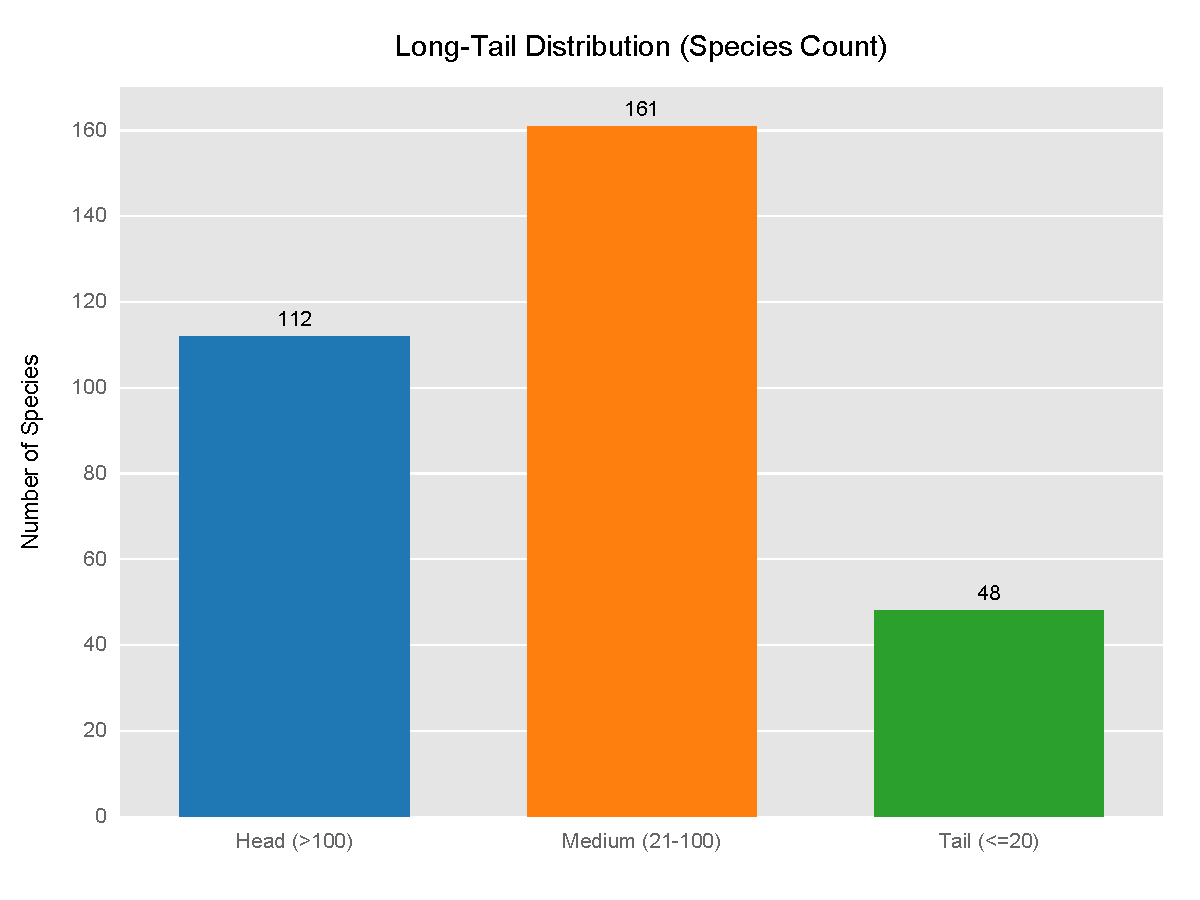
\includegraphics[width=0.75\linewidth,keepaspectratio]{figure1.pdf}
\caption{Long Tail distribution}
\label{fig:figure1}
\end{figure}

As shown in Table~\ref{tab:long-tail-analysis}, although 112 head species containing 82\% of the
total training samples, many of the species are represented by small
number of observations, which results in an increase of difficulty of
fine-grained recognition \citep{ref15}.

\footnotesize\setlength{\tabcolsep}{3pt}
\begin{longtable}[]{@{}
  >{\raggedright\arraybackslash}p{(\columnwidth - 6\tabcolsep) * \real{0.2499}}
  >{\raggedright\arraybackslash}p{(\columnwidth - 6\tabcolsep) * \real{0.2499}}
  >{\raggedright\arraybackslash}p{(\columnwidth - 6\tabcolsep) * \real{0.2501}}
  >{\raggedright\arraybackslash}p{(\columnwidth - 6\tabcolsep) * \real{0.2501}}@{}}
\caption{Long-Tail Analysis}\\
\toprule\noalign{}
\begin{minipage}[b]{\linewidth}\raggedright
Group
\end{minipage} & \begin{minipage}[b]{\linewidth}\raggedright
Species
\end{minipage} & \begin{minipage}[b]{\linewidth}\raggedright
Images
\end{minipage} & \begin{minipage}[b]{\linewidth}\raggedright
Percentage
\end{minipage} \\
\midrule\noalign{}
\endhead
\bottomrule\noalign{}
\endlastfoot
Head (\textgreater100) & 112 & 41,406 & 81.97\% \\
Medium (21-100) & 161 & 8,321 & 16.47\% \\
Tail (\textless=20) & 48 & 786 & 1.56\% \\
\end{longtable}
\makeatletter\edef\@currentlabel{\thetable}\def\@currentlabelname{Long-Tail Analysis}\makeatother
\label{tab:long-tail-analysis}
\normalsize\setlength{\tabcolsep}{6pt}

\section{Proposed Method}\label{proposed-method}

This paper proposes Bio-TAC, a taxonomy-aware multi-context
classifier for fine-grained fish species recognition on the OzFish
benchmark. The architecture in this section is presented using its
baseline training configuration, while alternative training and
adaptation strategies are evaluated experimentally in the later
sections. Bio-TAC is built on a DINOv3 backbone
\citep{ref25} that encodes four visual streams:
the ROI view of the target fish, and the three progressively wider
contextual views corresponding to the 3x, 5x, and full-frame scales
\citep{ref26}.

The MCEAM layer \citep{ref26} then fuses the
target-fish representation with information from the three wider context
views, producing a context-aware embedding. A learned gating mechanism
then controls the relative contribution of context-aware and ROI-only
representations before species classification.

\subsection{Context-Stream
Representation}\label{context-stream-representation}

For each target fish, four image streams are extracted from the complete
frame using its bounding box \emph{b = x, y, w, h}
\citep{ref26}. All local crops share the same
bounding-box center. The ROI stream is the original bounding-box crop,
representing the target fish's morphology. It may preserve
discriminative features such as body shape, fin structure, and visible
patterns, among other physical traits. The 3x context stream enlarges
the bounding-box's width and height by a factor of three. While it
contains the target fish, it also contains its immediate surroundings
and may provide beneficial information about nearby fish and specific
schooling patterns. The 5x context stream provides a wider view that may
include habitat-associated contextual cues such as coral, sand, rocks,
and reef structures. The full-frame stream provides global scene
information, giving full context from the entire provided frame. The
extracted views are processed using the common preprocessing and
augmentation pipeline described in later sections.\RL{}

\subsection{DinoV3 Encoder}\label{dinov3-encoder}

The four visual streams are encoded by a shared DINOv3 ViT-B/16 backbone
\citep{ref25,ref36}. Each 224x224 image is split into
16x16 patches, producing a 14x14 grid of 196 image patches. The backbone
represents each token using a 768-dimensional embedding and produces CLS
and patch-token representations for each stream. The CLS token is used
as the target fish representation, while the patch tokens provide
additional contextual features. The encoder weights are shared across
all four streams, ensuring that the target and contextual features are
represented within a common embedding space. The DINOv3 backbone is
initialized from pretrained weights \citep{ref25}
and kept frozen in the baseline formulation, while the downstream
fusion, projection, gating, and classification components are optimized
on the OzFish training set.

\subsection{Multi-Context Attention
Fusion}\label{multi-context-attention-fusion}

The Multi-Context Environmental Attention Module (MCEAM)
\citep{ref26} fuses the ROI representation with
features from the three wider context streams. The ROI CLS token is used
as the query, as it represents the target fish, while the patch tokens
from each context stream are used as keys and values, since they
represent candidate contextual regions that the ROI representation may
attend to, based on how useful the information is.

For context stream \emph{k}, the attended representation is calculated
as:

\begin{equation}
a^{(k)} = \operatorname{softmax}\left(\frac{\mathbf{Q}\bigl(\mathbf{K}^{(k)}\bigr)^{\mathsf{T}}}{\sqrt{d_h}}\right)\mathbf{V}^{(k)}
\label{eq:context-attention}
\end{equation}

where \emph{Q} is obtained from the ROI CLS token,
\(\left( K^{(k)} \right)\) and \(\left( V^{(k)} \right)\) are obtained
from the patch tokens of context stream \emph{k}, and \(d_{h}\) is the
feature dimension of each attention head. The module uses eight
attention heads and produces one attended representation for each of the
three context streams.

The three attended context representations are concatenated with the
original ROI representation. Since each representation contains 768
features, the concatenated vector has 3,072 dimensions. A feedforward
fusion network then projects this vector into a 256-dimensional
context-aware embedding, denoted by \(z_{context}.\)

To preserve a direct target-only representation, the ROI CLS token is
also independently projected into a 256-dimensional ROI embedding,
denoted by \(\left( z_{ROI} \right)\). A learned scalar gate determines
the relative contribution of the context-aware and ROI-only
representations for each sample. The final fused representation is
calculated as:

\begin{equation}
\mathbf{z} = g\mathbf{z}_{context} + (1-g)\mathbf{z}_{ROI}
\label{eq:gated-fusion}
\end{equation}

where \emph{g} is produced by a sigmoid function and has a value between
zero and one. A larger value of \emph{g} gives greater weight to the
context-aware representation, while a smaller value places greater
emphasis on the target fish itself. The resulting 256-dimensional
representation is subsequently passed to the species classification
head.

\subsection{Species Prediction and Taxonomic
Marginalization}\label{species-prediction-and-taxonomic-marginalization}

The final fused representation is passed through a linear classifier to
produce logits over the \emph{S} species classes:

\begin{equation}
\boldsymbol{\ell} = \mathbf{W}_{c}\mathbf{z} + \mathbf{b}_{c}
\label{eq:species-logits}
\end{equation}

The logits are then converted into species probabilities using softmax:

\begin{equation}
p(s_i) = \frac{\exp(\ell_i)}{\sum_{j=1}^{S}\exp(\ell_j)}
\label{eq:species-softmax}
\end{equation}

The proposed model uses a single species-level prediction head. The
genus and family probabilities get derived from the species distribution
using known taxonomic relationships. For a certain genus \emph{g}, the
probabilities of all species that belong to that genus are summed:

\begin{equation}
p(g) = \sum_{s:\operatorname{genus}(s)=g} p(s)
\label{eq:genus-marginalization}
\end{equation}

Similarly, the probability of a family f is obtained by:

\begin{equation}
p(f) = \sum_{s:\operatorname{family}(s)=f} p(s)
\label{eq:family-marginalization}
\end{equation}

This marginalization process makes sure that the species, genus, and
family level probabilities stay consistent taxonomy-wise
\citep{ref24,ref61}. All higher-level probabilities are
derived from the same species distribution, unlike other methods that
use separate prediction heads for each taxonomic level
\citep{ref23,ref26,ref60}.

\subsection{Taxonomy-Aware Training
Objective}\label{taxonomy-aware-training-objective}

The OzFish training set has a long-tailed distribution, with large
differences in the number of samples for each species. The species-level
objective uses class-balanced (CB) focal loss
\citep{ref14,ref63} to reduce the dominance of very
frequent classes.

For species \emph{c} with \emph{n\textsubscript{c}} training samples, an
effective-number weight is first calculated
as\citep{ref14}:

\begin{equation}
\alpha_c = \frac{1-\beta}{1-\beta^{n_c}}.
\label{eq:effective-number-weight}
\end{equation}

The values are normalized across all of the species to obtain a final
class weight \emph{w\textsubscript{c}}. Rare species therefore receive
relatively greater weight than frequently observed species.

For a sample with true species \emph{y}, the species-level loss is
defined as \citep{ref14,ref63}:

\begin{equation}
\mathcal{L}_{species} = -w_y\left(1-p(s_y)\right)^{\gamma}\log p(s_y),
\label{eq:species-loss}
\end{equation}

where \emph{p(s\textsubscript{y})} is the probability that's assigned to
the correct species and \(\gamma\) reduces the contribution of examples
that have already been classified with high confidence. The values for β
and \(\gamma\) are set as 0.9999 and 2 respectively
\citep{ref14,ref63}.

The marginalized genus and family distributions provide additional
supervision:

\begin{equation}
\mathcal{L}_{genus} = -\log p(g_y),
\label{eq:genus-loss}
\end{equation}

\begin{equation}
\mathcal{L}_{family} = -\log p(f_y),
\label{eq:family-loss}
\end{equation}

where \emph{g\textsubscript{y }}and \emph{f\textsubscript{y}} denote the
true genus and family that's associated with species \emph{y}.

The complete training objective is:

\begin{equation}
\mathcal{L} = \lambda_s\mathcal{L}_{species} + \lambda_g\mathcal{L}_{genus} + \lambda_f\mathcal{L}_{family},
\label{eq:training-objective}
\end{equation}

with reference weights set to:

\(\lambda_{s} = 1,\ \lambda_{g} = 2,\ \lambda_{f} = 3\).

The genus and family level terms encourage the predicted probability
mass to stay within the correct higher-level taxonomic groups, while the
CB focal term addresses the great imbalance between common and rare
species that is found in OzFish.

\section{Benchmark Protocol and Experimental
Setup}\label{benchmark-protocol-and-experimental-setup}

This section describes the benchmark comparison protocol, training and
implementation settings, evaluation metrics, and ablation design used in
the experiments. The experimental setup was designed to provide
consistent comparisons across the evaluated models while accommodating
method-specific requirements wherever it was deemed necessary.

\subsection{Benchmark Models and Comparison
Protocol}\label{benchmark-models-and-comparison-protocol}

For this benchmark paper, we evaluated 8 different models representing
different architectural families on the OzFish benchmark for comparison.
The conventional CNN baselines selected for this benchmark include
ResNet-50 \citep{ref39}, ConvNeXt-Tiny
\citep{ref41}, and EfficientNetV2-S
\citep{ref40}, while the transformer-based models
are ViT-B/16 \citep{ref36} and Swin-B
\citep{ref38}. We also included DINOv3 ViT-B/16
linear probe, a self-supervised representation baseline
\citep{ref25}, as well as MATANet, which provides
a specialized fine-grained and context-aware comparison
\citep{ref26}. Finally, Bio-TAC which is our
proposed taxonomy-aware multi-context approach.

The comparison protocol for the different architectures follows a
specific ruleset necessary for the benchmark. There were some common
aspects across the evaluation of all models to maintain consistency
across the experiments, such as the train/val/test split which was kept
consistent, as well as the metrics that were used to evaluate each
model's performance. The experimental conditions were standardized
wherever possible, and every model solves the same species
classification task. There were, however, some method-specific
differences that remained due to each model's differing design and
architecture.

There is an important distinction between the standard baselines and
Bio-TAC, however, as all of the single crop baselines rely solely
on the ROI crop, meaning that it primarily focuses on the target fish
morphology, while Bio-TAC has access to the target morphology as
well as the surrounding visual information taken from the 3 extra visual
crops, therefore feeding more information to Bio-TAC in comparison
to the other single-crop baselines. This distinction is important when
interpreting the benchmark results, as we are comparing complete
classification systems against each other instead of isolating the
effect of any single architectural component. The contribution of the
extra context streams is separately examined through the ablation
experiments that are described in Section~\ref{ablation-protocol}.

One exception to the rest of the models is MATANet
\citep{ref26}. Since MATANet\textquotesingle s
official implementation was released by its authors, it was used
directly rather than being reimplemented. We used the same OzFish
benchmark split and converted the samples into the format that
MATANet\textquotesingle s code expects, then we trained MATANet using
its intended architecture and native training procedure to then evaluate
the produced species predictions using the common benchmark evaluation
metrics. MATANet was not forced to follow the common training
configuration since there are method-specific details that may not be
common with the other model implementations.

\subsection{Training and Implementation
Details}\label{training-and-implementation-details}

Unless otherwise specified, the following preprocessing and training
settings apply to models implemented within the common benchmark
framework. MATANet retained its native implementation and training
procedure as described separately below
\citep{ref26}. Before the images were passed to
the models, they had to be prepared using preprocessing and augmentation
methods. The images were all converted into a standardized 224x224 input
resolution. aspect-ratio-preserving letterbox resizing was used to
preserve the morphology of the target fish without distorting its aspect
ratio, with bicubic interpolation used during resizing and zero padding
added wherever necessary to obtain the required square input. The RGB
images that resulted from this preprocessing were then normalized using
the standard ImageNet mean and standard deviation. data augmentation was
also introduced during training to increase the variation in fish
orientation and underwater image appearance. Geometric augmentation
consisted of horizontal flipping and rotations between -30 degrees and
+30 degrees, while vertical flipping was excluded, as it would produce
orientations that are uncommon in the original imagery. We included
additional appearance-based perturbations like synthetic marine-snow
artifacts, motion blur, Gaussian noise, and some brightness, contrast,
and saturation changes. For Bio-TAC, the same geometric
transformation was applied to all the four visual streams to preserve
spatial consistency. There was no stochastic augmentation applied during
validation or testing.

The models implemented within the common benchmark framework were
trained with a 60-epoch budget using the AdamW optimizer. A fixed batch
size of 32 was used, as well as a weight decay of 0.01 and a learning
rate of 1x10\textsuperscript{-4}, with the exception of Bio-TAC's
learning rate being 1x10\textsuperscript{-5} to provide more
conservative updates during the full fine-tuning of the pretrained
DINOv3 backbone. A three-epoch warm-up period was used rather than
applying the full learning rate from the beginning, during which the
learning rate was increased gradually to its configured value. After the
warm-up period, the learning rate gets progressively reduced using a
cosine annealing schedule for the remaining portion of the training
period. To reduce GPU memory requirements and improve computational
efficiency, we also implemented automatic mixed-precision training.

The pretrained backbones had differing treatment across the evaluated
models. Regarding the DINOv3 linear-probe baseline
\citep{ref25}, its backbone remained frozen
throughout the training period, and only the species-classification
layer was optimized. Contrastingly, the pretrained ResNet-50
\citep{ref39}, EfficientNetV2-S
\citep{ref40}, ConvNeXt-Tiny
\citep{ref41}, ViT-B/16
\citep{ref36}, and Swin-B
\citep{ref38} baselines were fine-tuned
end-to-end on the OzFish training set. As for Bio-TAC, the
pretrained DINOv3 backbone \citep{ref25} was
fine-tuned jointly with the MCEAM module
\citep{ref26}, projection layers, gating
mechanism, and species-classification head, which allows for both the
visual representation as well as the newly introduced components to
adapt to the OzFish classification task.

We maintained an exponential moving average (EMA) of the trainable model
parameters throughout training using a decay coefficient of 0.999, which
was also used during validation. At the end of each epoch, the model was
evaluated on the validation partition, and the checkpoint that had
achieved the lowest validation Mean Hierarchical Distance (MHD)
\citep{ref24,ref30} was retained as the best-performing
checkpoint. MHD was used consistently as the predefined
checkpoint-selection criterion, while the complete set of classification
and taxonomy-aware metrics was reported on the test partition. We did
not apply early stopping, meaning that all of the models completed the
full 60-epoch training schedule regardless of whether or not the score
started declining after it reached the best validation performance. The
retained checkpoint was used for final evaluation on the test partition
after the training had completed.

To account for the stochastic nature of model training, each
configuration was trained independently using three random seeds: 0, 1,
2. The train/val/test partitions remained fixed across all of the runs,
which meant that the different seeds only affected the stochastic
training operations, such as parameter initialization, data ordering,
and data augmentation, allowing for the assessment of the stability of
each model without introducing variation from different dataset
partitions. The experimental configurations were stored in YAML files,
with the software environment and source-code revision recorded,
supporting reproducibility.

MATANet's implementation has its own specific training procedure, and it
was treated separately from the models trained within the common
benchmark framework \citep{ref26}. The model was
trained using a DINOv2-Large backbone
\citep{ref47} with an input resolution of
256x256. The model had an effective batch size of 16, a learning rate of
1x10\textsuperscript{-6}, and a weight decay of 0.001 over a 60-epoch
training schedule. The native data transformations as well as the
hierarchical training procedure for MATANet were retained, while the
same OzFish benchmark partition and common evaluation metrics were used,
thus ensuring that the final predictions it generates stayed comparable
with the other evaluation methods.

\subsection{Evaluation Metrics and Statistical
Reporting}\label{evaluation-metrics-and-statistical-reporting}

Due to the strong long-tailed class distribution
\citep{ref15,ref16} and hierarchical taxonomy
\citep{ref23,ref24} of the OzFish benchmark, we
evaluated model performance using several complementary metrics.
Conventional classification metrics were used as a way to quantify
species-level recognition performance. Taxonomy-aware metrics were also
used to assess the severity within the taxonomic hierarchy of any
incorrect prediction. Performance was examined separately across head,
medium, and tail species to determine how well each evaluated model
dealt with varying levels of training-data availability. All benchmark
results are reported as the mean ± standard deviation across the three
independent runs described in Section~\ref{training-and-implementation-details}.

\subsubsection{Classification
Performance}\label{classification-performance}

To determine the performance of classification for each evaluated model,
three different accuracy metrics were used: Macro Accuracy, top-1
accuracy, and top-5 accuracy. Since OzFish has a long-tailed class
distribution, overall accuracy metrics may favour frequent species,
therefore Macro Accuracy was used as the primary class-balanced
species-level performance metric reported in the benchmark in order to
give equal importance to each of the species by first calculating the
accuracy separately for each species and then averaging the species
accuracies \citep{ref16,ref65}. The formula for Macro Accuracy is
as follows:
\begin{equation}
\mathrm{MacroAcc} = \frac{1}{C}\sum_{c=1}^{C}\frac{TP_c}{N_c},
\label{eq:macro-accuracy}
\end{equation}

Where C represents the number of evaluated species, TP\textsubscript{c}
represents the number of correctly classified samples belonging to
species c, and N\textsubscript{c} represents the total test samples
belonging to species c.

Top-1 accuracy was also used as a classification metric to measure if
the highest scoring species out of all predictions made by the evaluated
models is correct. Top-1 is sample-weighted rather than class-balanced,
as every sample has equal influence.

Top-5 accuracy was utilized to measure if the ground-truth species was
among the five highest scoring species predictions that the evaluated
model produced. Since fine-grained classification involves visually
similar species, the model may assign high probability to several
plausible closely related classes, which is why top-5 accuracy proves a
useful complementary metric in the case that the model assigned the
ground-truth species one of its five highest scores, even if it wasn't
ranked first.

\subsubsection{Taxonomy-Aware
Performance}\label{taxonomy-aware-performance}

Taxonomic error severity was evaluated using a hierarchical error score
based on the family-genus-structure of the OzFish benchmark
\citep{ref24,ref30,ref61}. For a ground-truth species
\emph{y} and predicted species \(\widehat{y}\), the hierarchical
distance is defined as:

\begin{equation}
d(y,\widehat{y}) = \begin{cases}
0, & \widehat{y}=y, \\
1, & \widehat{y}\neq y,\ \text{same genus}, \\
2, & \text{different genera within the same family}, \\
3, & \text{the species belong to different families}.
\end{cases}
\label{eq:hierarchical-distance}
\end{equation}

MHD was then calculated by averaging this score over all test samples:

\begin{equation}
\mathrm{MHD} = \frac{1}{N}\sum_{i=1}^{N} d(y_i,\widehat{y}_i),
\label{eq:mean-hierarchical-distance}
\end{equation}

Where N is the number of test samples, \(y_{i}\) is the ground-truth
species for sample \emph{i}, and \({\widehat{y}}_{i}\) is the
corresponding predicted species. A lower MHD value indicates better
overall taxonomic performance, resulting from a combination of more
correct predictions and errors that remain closer to the ground-truth
species within the taxonomic hierarchy.

Another metric that was used was Mean Mistake Severity (MMS), as it was
used to isolate the severity of incorrect predictions
\citep{ref24}. Unlike MHD, correctly classified
samples are excluded from this calculation, meaning that the metric only
measures the average taxonomic distance of the mistakes made by the
model.

Genus and family accuracy were additionally reported by checking whether
the top-1 predicted species belonged to the same genus or family as the
ground-truth species.

\subsubsection{Long-Tail
Performance}\label{long-tail-performance}

As the OzFish benchmark follows a long-tailed class distribution, it was
important to also evaluate model performance according to the number of
training samples available for each species. For benchmark-specific
long-tail analysis, species were divided into three frequency groups
based on their training-set sample counts, with head species containing
more than 100 training samples, medium species containing between 21 and
100 samples, and tail species containing 20 or fewer samples
\citep{ref16}.

Performance within each group was calculated using Macro Accuracy
computed separately for the species belonging to that group, where the
accuracy of each species was independently calculated before averaging
across the species that belonged to the corresponding frequency group.
This prevents more frequently represented species within a certain group
from having a greater influence on the reported value. The resulting
accuracies of the head, medium, and tail groups provide a more detailed
view of how each evaluated model performs under different levels of
training-data availability, particularly for rare species where limited
training data makes recognition more challenging
\citep{ref15,ref16}.

\subsection{Ablation Protocol}\label{ablation-protocol}

A series of matched ablation experiments was conducted to further
examine the principal architecture and training choices of Bio-TAC.
The ablations were organized into controlled comparison groups rather
than treating every experiment as a direct modification of a single
reference configuration. Within each comparison group, all experimental
settings were fixed except for the factor that was under investigation.

The contribution of the multi-context pathway was examined under a fixed
frozen-DINOv3 configuration. The complete three-context MCEAM
configuration \citep{ref26} was compared with an
ROI-only variant, where both the contextual streams and the MCEAM were
removed. A variant with reduced-context that retained only the 3x
contextual stream was also compared with the complete 3x, 5x, and
full-frame configuration as a way to examine the contribution of the
multi-scale contextual information. Under the same configuration, the
depth of MCEAM varied between one, two, and four attention blocks.

The backbone adaptation was evaluated separately at a fixed learning
rate of 1x10\textsuperscript{-4}\citep{ref51} The
frozen DINOv3 encoder was compared with configurations in which the
final two transformer blocks, the final four blocks, or the complete
backbone were trainable. A separate learning-rate comparison was
subsequently performed for the fully fine-tuned backbone using
1x10\textsuperscript{-4} and 1x10\textsuperscript{-5}.

The effects of taxonomy-aware supervision and species-level loss
formulation were evaluated under the fully fine-tuned DINOv3
configuration using a matched 2x2 objective design. The species-level
objective used either CB focal loss \citep{ref14,ref63} or conventional cross entropy,
while hierarchical supervision \citep{ref24,ref26} was independently enabled or
disabled, allowing the contribution of hierarchical supervision and
class-imbalance-aware loss to be examined separately while still
retaining the same architecture and training configuration.

Finally, a separate matched backbone comparison replaced DINOv3
\citep{ref25} with DINOv2
\citep{ref47} while retaining the remaining
full-fine-tuning configuration. Since the corresponding DINOv2 and
DINOv3 encoders are not architecturally identical, this experiment is
interpreted as a comparison of pretrained backbones rather than a strict
isolation of the pretraining method.

\section{Results and Discussion}\label{results-and-discussion}

The analysis and presentation of the experimental results obtained on
the proposed OzFish benchmark are presented in this section. Starting
the analysis with the comparison between the main classification models,
followed by frequency-group performance, comparison with MATANet,
ablation studies, qualitative analysis, computational efficiency, and
finally a summary of the overall analysis.

\subsection{Main Benchmark Results}\label{main-benchmark-results}

This section presents the results of all the tested methods on the
proposed OzFish benchmark. Results are reported as mean ± standard
deviation over three independent seeds. The evaluation includes Macro
Accuracy, Top-1, MHD, MMS, and cumulative Genus- and Family-level
Accuracy, as shown in Table~\ref{tab:main-results}.

\begin{table}[H]
\centering
\caption{Performance comparison of the evaluated models on the OzFish benchmark. The best score in each column is shown in bold, and the second-best score is underlined.}\label{tab:main-results}
\footnotesize
\begin{tabular*}{\textwidth}{@{\extracolsep{\fill}}lcccc@{}}
\toprule
Model & Macro Accuracy & Top-1 & MHD & MMS \\
\midrule
Linear Probe & 0.471±0.002 & 0.675±0.001 & 0.764±0.003 & 2.349±0.001 \\
ResNet-50 & 0.571±0.007 & 0.749±0.002 & 0.539±0.005 & 2.145±0.006 \\
EfficientNetV2-S & 0.624±0.013 & 0.782±0.005 & 0.447±0.010 & 2.054±0.006 \\
ConvNeXt-T & 0.662±0.002 & 0.809±0.003 & 0.373±0.004 & 1.948±0.016 \\
ViT-B & 0.658±0.010 & 0.808±0.005 & 0.377±0.011 & 1.966±0.006 \\
Swin-B & 0.689±0.009 & 0.820±0.003 & 0.347±0.008 & 1.931±0.019 \\
MATANet & \textbf{0.692±0.012} & \textbf{0.844±0.002} & \textbf{0.288±0.008} & \textbf{1.843±0.059} \\
\textbf{Proposed Model} & \uline{0.690±0.023} & \uline{0.842±0.006} & \uline{0.291±0.008} & \uline{1.844±0.018} \\
\bottomrule
\end{tabular*}

\vspace{6pt}

\begin{tabular*}{\textwidth}{@{\extracolsep{\fill}}lcc@{}}
\toprule
Model & Genus Accuracy & Family Accuracy \\
\midrule
Linear Probe & 0.754±0.001 & 0.807±0.001 \\
ResNet-50 & 0.833±0.002 & 0.879±0.002 \\
EfficientNetV2-S & 0.866±0.002 & 0.905±0.002 \\
ConvNeXt-T & 0.890±0.001 & 0.928±0.001 \\
ViT-B & 0.888±0.004 & 0.927±0.002 \\
Swin-B & 0.900±0.002 & 0.933±0.003 \\
MATANet & \textbf{0.917±0.006} & \uline{0.951±0.003} \\
\textbf{Proposed Model} & \uline{0.916±0.002} & \textbf{0.951±0.001} \\
\bottomrule
\end{tabular*}
\end{table}

As the backbone of conventional image classification baselines become
more capable, they show a consistent improvement. Where ResNet-50
\citep{ref39} achieves a Macro Accuracy of 0.571,
while EfficientNetV2-S \citep{ref40} and
ConvNeXt-T \citep{ref41} increase this to 0.624
and 0.662, respectively. A similar performance is seen with
transformer-based baselines, with ViT-B achieving 0.658
\citep{ref36} and Swin-B
\citep{ref38} reaching 0.689 Macro Accuracy. The
trend shows that the benchmark remains difficult enough for performance
to be affected by differences in visual representation capabilities.

The proposed model achieves a macro accuracy of 0.690 and a Top-1
accuracy of 0.842, making it competitive with the strongest benchmark
baselines. More importantly, it achieves a MHD of 0.291 and MMS of
1.844, together with Genus and Family accuracies of 0.916 and 0.951,
respectively. These results show that, in addition to producing accurate
species prediction, the proposed method tends to make taxonomical closer
mistakes when its prediction is incorrect.

The results also show that Top-1 accuracy alone is not enough to
describe the model quality, because the benchmark is fine-grained and
taxonomically structured. Since models with similar Top-1 accuracy score
can have huge difference in the severity of their classification errors,
therefore, encouraging the use of hierarchical evaluation metrics in
addition to traditional accuracy metrics
\citep{ref24}.

\subsection{Performance Across Frequency
Groups}\label{performance-across-frequency-groups}

\footnotesize\setlength{\tabcolsep}{3pt}
\begin{longtable}[]{@{}
  >{\raggedright\arraybackslash}p{(\columnwidth - 6\tabcolsep) * \real{0.2500}}
  >{\raggedright\arraybackslash}p{(\columnwidth - 6\tabcolsep) * \real{0.2500}}
  >{\raggedright\arraybackslash}p{(\columnwidth - 6\tabcolsep) * \real{0.2500}}
  >{\raggedright\arraybackslash}p{(\columnwidth - 6\tabcolsep) * \real{0.2500}}@{}}
\caption{Macro Accuracy across head, medium, and tail species groups, defined by training-set frequency. The best score in each column is shown in bold, and the second-best score is underlined.}\label{tab:frequency-results}\\
\toprule\noalign{}
\begin{minipage}[b]{\linewidth}\raggedright
model
\end{minipage} & \begin{minipage}[b]{\linewidth}\raggedright
Head
\end{minipage} & \begin{minipage}[b]{\linewidth}\raggedright
Medium
\end{minipage} & \begin{minipage}[b]{\linewidth}\raggedright
Tail
\end{minipage} \\
\midrule\noalign{}
\endhead
\bottomrule\noalign{}
\endlastfoot
Linear Probe & 0.629±0.003 & 0.430±0.003 & 0.260±0.005 \\
ResNet-50 & 0.730±0.005 & 0.517±0.001 & 0.397±0.030 \\
EfficientNetV2-S & 0.779±0.002 & 0.577±0.009 & 0.441±0.060 \\
ConvNeXt-T & 0.804±0.003 & 0.628±0.009 & 0.467±0.014 \\
ViT-B & 0.803±0.002 & 0.625±0.014 & 0.460±0.015 \\
Swin-B & 0.817±0.001 & 0.656±0.012 & \textbf{0.521±0.018} \\
MATANet & \uline{0.821±0.004} & \textbf{0.681±0.017} & \uline{0.466±0.017} \\
\textbf{Proposed Model} & \textbf{0.843±0.004} & \uline{0.668±0.008} &
0.444±0.110 \\
\end{longtable}
\normalsize\setlength{\tabcolsep}{6pt}

To further examine the effect of the long-tailed species distribution,
Table~\ref{tab:frequency-results} reports the macro accuracy across frequency groups Head, Medium,
and Tail according to their training-set frequency
\citep{ref16}. A more detailed understanding of
whether the overall benchmark performance can be a representative of
both the common and rare species is provided by this analysis.

As the species frequency decreases, a performance decline is noted
across all models, indicating that classifying rare species is still
substantially more difficult than classification of frequently observed
species \citep{ref10,ref15}. The proposed model performs well
on the head and medium frequency species with a macro accuracy of 0.843
and 0.668, respectively, while its tail performance remains unstable
with a macro accuracy of 0.444. This shows that even with the
improvements attained by the proposed architecture, challenges connected
to limited training samples are still not completely eliminated. The
frequency group results showcase a crucial exchange in the proposed
model. It achieved the highest head group frequency performance compared
to the remaining models and keeps close performance in medium group
frequency species. The tail group result, on the other side, is lower
and shows significantly greater variance among seeds. This indicates
that while extremely rare species continue to be a significant benchmark
limitation, the suggested architecture is effective for the dominating
and moderately represented classes.

\subsection{Comparison with MATANet}\label{comparison-with-matanet}

MATANet \citep{ref26}, introduced in Section~\ref{environmental-context-in-marine-recognition},
is the closest context- and taxonomy-aware comparator. Therefore, the
comparison is considered useful for determining whether the proposed
approach brings competitive performance under the same benchmark
conditions.

The proposed model and MATANet show very similar performance across the
reported evaluation metrics. The proposed model obtains a Macro Accuracy
of 0.690 compared with 0.692 for MATANet, while Top-1 Accuracy is 0.842
compared with 0.844. Their MHD are similarly close, at 0.291 for the
proposed model and 0.288 for MATANet. Genus- and family-level accuracies
are also nearly identical, reaching 0.916 and 0.951 for the proposed
model, compared with 0.917 and 0.951 for MATANet.

These comparable results are obtained despite differences in model
scale. MATANet uses a fine-tuned DINOv2 large backbone
\citep{ref47}, on the other hand, the proposed
model employs a smaller DINOv3 based backbone
\citep{ref25} together with multi-context
attention and hierarchical supervision. Therefore, the proposed model
reached a similar performance of classification and taxonomic
consistency while running with a substantially smaller backbone.

In conclusion, the results indicate that the proposed model offers a
competitive alternative to MATANet on the benchmark, with the main
difference not coming from a significant difference in overall accuracy
but rather from the balance between predictive performance and model
scale.

\subsection{Ablation Studies}\label{ablation-studies}

The ablation studies look into the specific aspects and design choices
that make up the proposed model. The internal experimental
configurations utilized to separate the impacts of backbone adaptation,
contextual modeling, hierarchical supervision, and long-tail methods are
included in this section, in contrast to the primary benchmark
comparison.

\subsubsection{Backbone Adaptation}\label{backbone-adaptation}

The impact of adapting the task-specific backbone is first assessed by
increasing the number of trainable blocks inside the pretrained DINOv3
backbone \citep{ref25}. As shown in Figure~\ref{fig:figure2},
just from unfreezing the last two blocks, the Macro Accuracy increases
from 0.507 ± 0.006 to 0.618 ± 0.006 and reduces MHD from 0.632 ± 0.012
to 0.421 ± 0.004. Further increasing the fine-tuning to the last four
blocks increases Macro Accuracy to 0.657 ± 0.008 and reduces MHD to
0.385 ± 0.008.

Finally, fine-tuning the full backbone further increases Macro Accuracy
to 0.677 ± 0.004 and reduces Mean Hierarchical Distance to 0.368 ±
0.003. The results indicate that increasing the number of backbone
adaptations significantly improves taxonomic error quality and species
classification \citep{ref51}.



\begin{figure}[H]
\centering
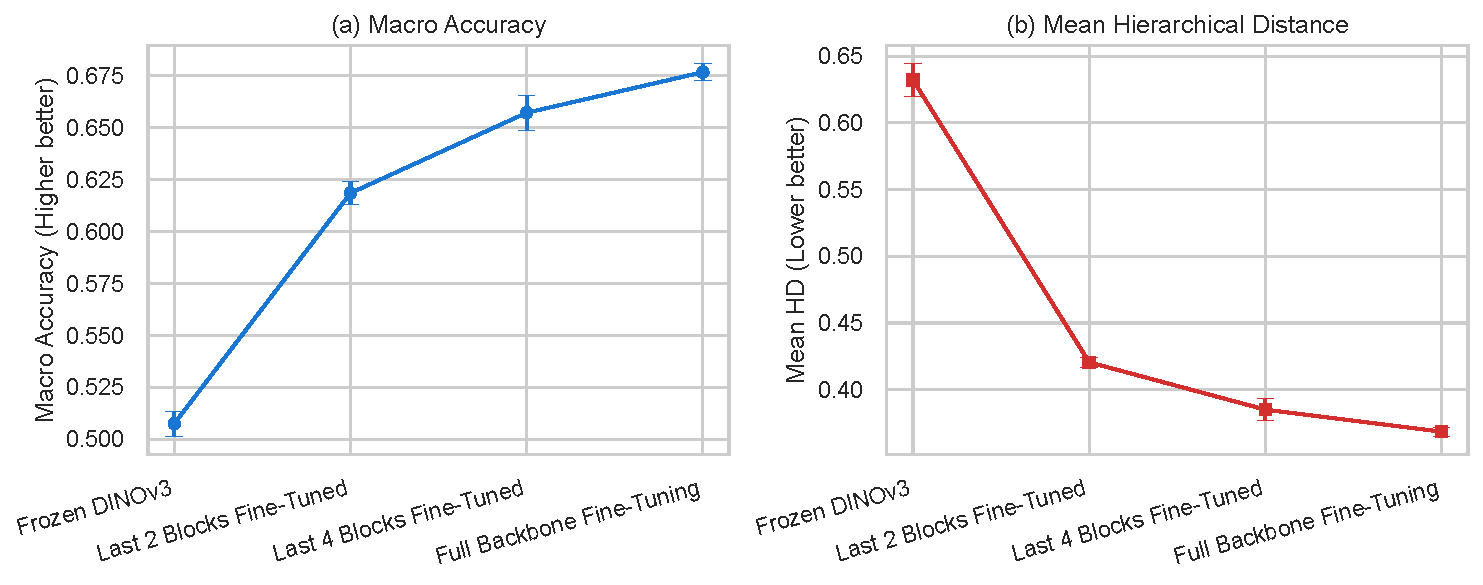
\includegraphics[width=\linewidth,keepaspectratio]{figure2.pdf}
\caption{Impact on fine-grained OzFish classification of progressive DINOv3 backbone adaptation. Results are reported as mean ± standard deviation over three seeds for a frozen backbone, fine-tuning of the last two blocks, fine-tuning of the last four blocks, and full backbone fine-tuning. (a) Macro Accuracy, (b) Mean Hierarchical Distance, where more taxonomically consistent errors are indicated by lower values.}
\label{fig:figure2}
\end{figure}



\subsubsection{Taxonomy-Aware
Objective}\label{taxonomy-aware-objective}

The effect of hierarchical supervision is evaluated by comparing flat
species-level classification with the taxonomy-aware objective under the
same unfrozen training settings. As shown in Figure~\ref{fig:figure3}, both produce
similar species level performance, with a Top-1 score of 0.844 ± 0.005
for the flat objective and 0.842 ± 0.006 for the taxonomy-aware
objective.

On the other hand, the difference is more shown in hierarchical
measures. The taxonomy-aware objective reduces MHD from 0.314 ± 0.011 to
0.291 ± 0.008 and MMS from 2.009 ± 0.025 to 1.844 ± 0.018. Family
Accuracy increases from 0.939 ± 0.003 to 0.951 ± 0.001, while Genus
Accuracy increases from 0.903 ± 0.004 to 0.916 ± 0.002.

The results show that rather than significant improvement in exact
species-level accuracy, the taxonomy-aware objective\textquotesingle s
main contribution is improved taxonomic consistency
\citep{ref24}. Therefore, while preserving
comparable species-level classification performance, integrating the
species, genus, and family relationship into the objective increases the
quality of incorrect predictions.



\begin{figure}[H]
\centering
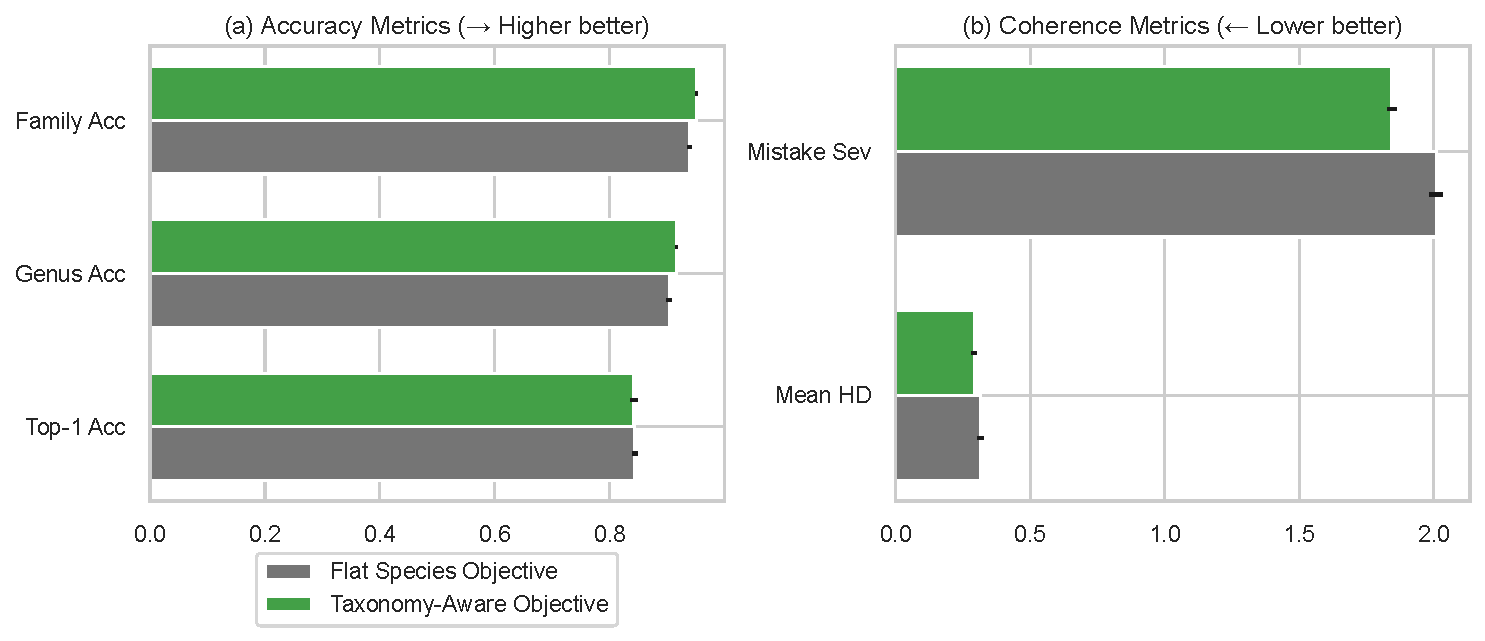
\includegraphics[width=\linewidth,keepaspectratio]{figure3.pdf}
\caption{Comparison of flat species-level and taxonomy-aware objectives. (a) Reports species and taxonomy level accuracy metrics, (b) reports MMS and MHD.}
\label{fig:figure3}
\end{figure}



\subsubsection{Context Modeling}\label{context-modeling}

By comparing the target fish representation with increasingly broader
spatial context, the influence of contextual visual information is
tested. The ROI only configuration includes tight fish crops without any
MCEAM based contextual streams, whereas the broader configuration uses
social and habitat information around the target fish.

Using the same frozen DINOv3 setting, as shown in Figure~\ref{fig:figure4}(a), ROI only
configuration achieves a Macro Accuracy of 0.466 ± 0.006, which
increases to 0.512 ± 0.002 when social context is introduced. While the
full-context configuration achieves a Macro Accuracy of 0.507 ± 0.006.
The results show that integrating contextual information does in fact
provide significant improvement rather than using the fish ROI only,
however, adding multiple contextual streams does not necessarily produce
an increase in Macro Accuracy.

Another thing that should be assessed is the effect of adding more MCEAM
attention depth, which is also tested using the same frozen DINOv3
settings and by Macro Accuracy metric. As shown in Figure~\ref{fig:figure4}(b), increasing
the depth from one to two attention blocks increases Macro Accuracy from
0.507 ± 0.006 to 0.512 ± 0.008, while increasing the depth to four
blocks reduces it to 0.505 ± 0.004. This implies that increasing the
depth does not correspond to improved classification performance.



\begin{figure}[H]
\centering
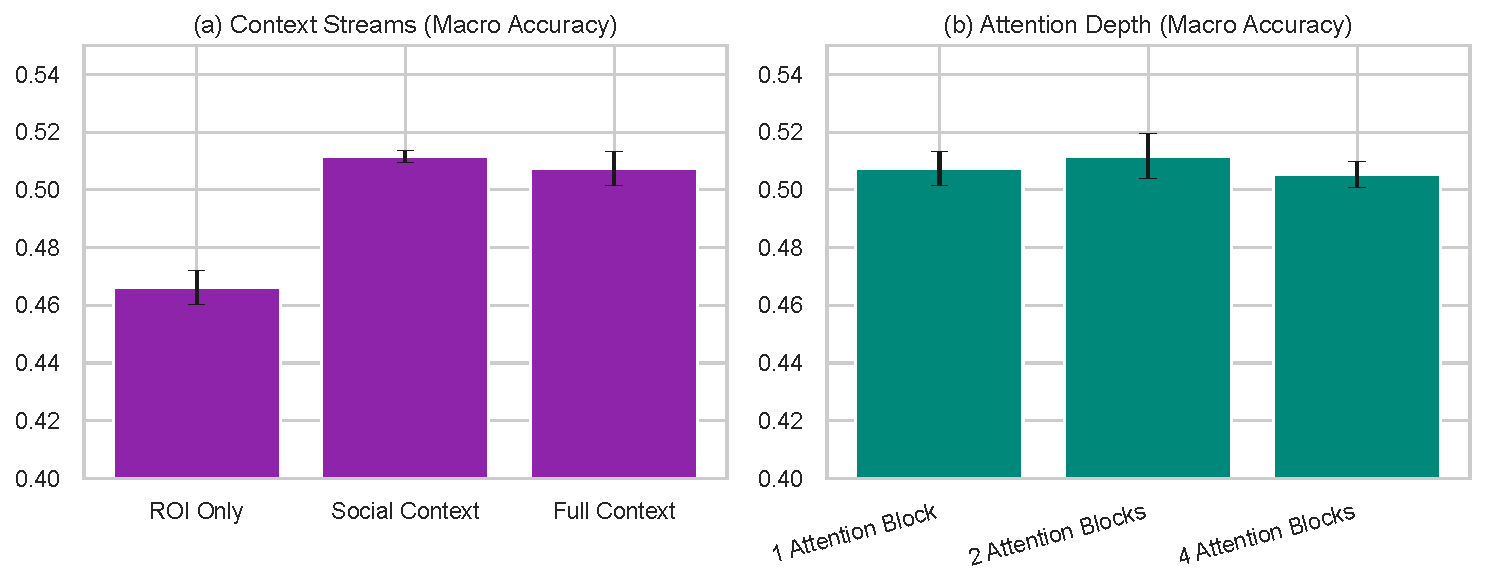
\includegraphics[width=\linewidth,keepaspectratio]{figure4.pdf}
\caption{Ablation of contextual representation and MCEAM depth under the frozen DINOv3 configuration. (a) Compares the different context configurations, from only ROI classification to broader contextual inputs. (b) Effect of increasing MCEAM attention depth from one to four blocks. Results are reported as mean ± standard deviation over three seeds.}
\label{fig:figure4}
\end{figure}



\subsubsection{Long-Tail Components}\label{long-tail-components}

In order to address the severe class imbalance in the OzFish dataset,
the evaluation across the head, medium, and tail frequency groups under
the frozen DINOv3 setting was needed to show the impact of different
sampling strategies and loss functions.

As shown in Figure~\ref{fig:figure5}(a), using balanced sampling rather than random
sampling slightly improves the performance on rare species, increasing
Macro Accuracy on the tail classes from 0.316 ± 0.044 to 0.328 ± 0.036,
and on the medium classes from 0.465 ± 0.005 to 0.481 ± 0.004. On the
other hand, this exchange comes with a noticeable cost to the dominant
species, reducing Macro Accuracy on the head classes from 0.660 ± 0.011
to 0.638 ± 0.009.



\begin{figure}[H]
\centering
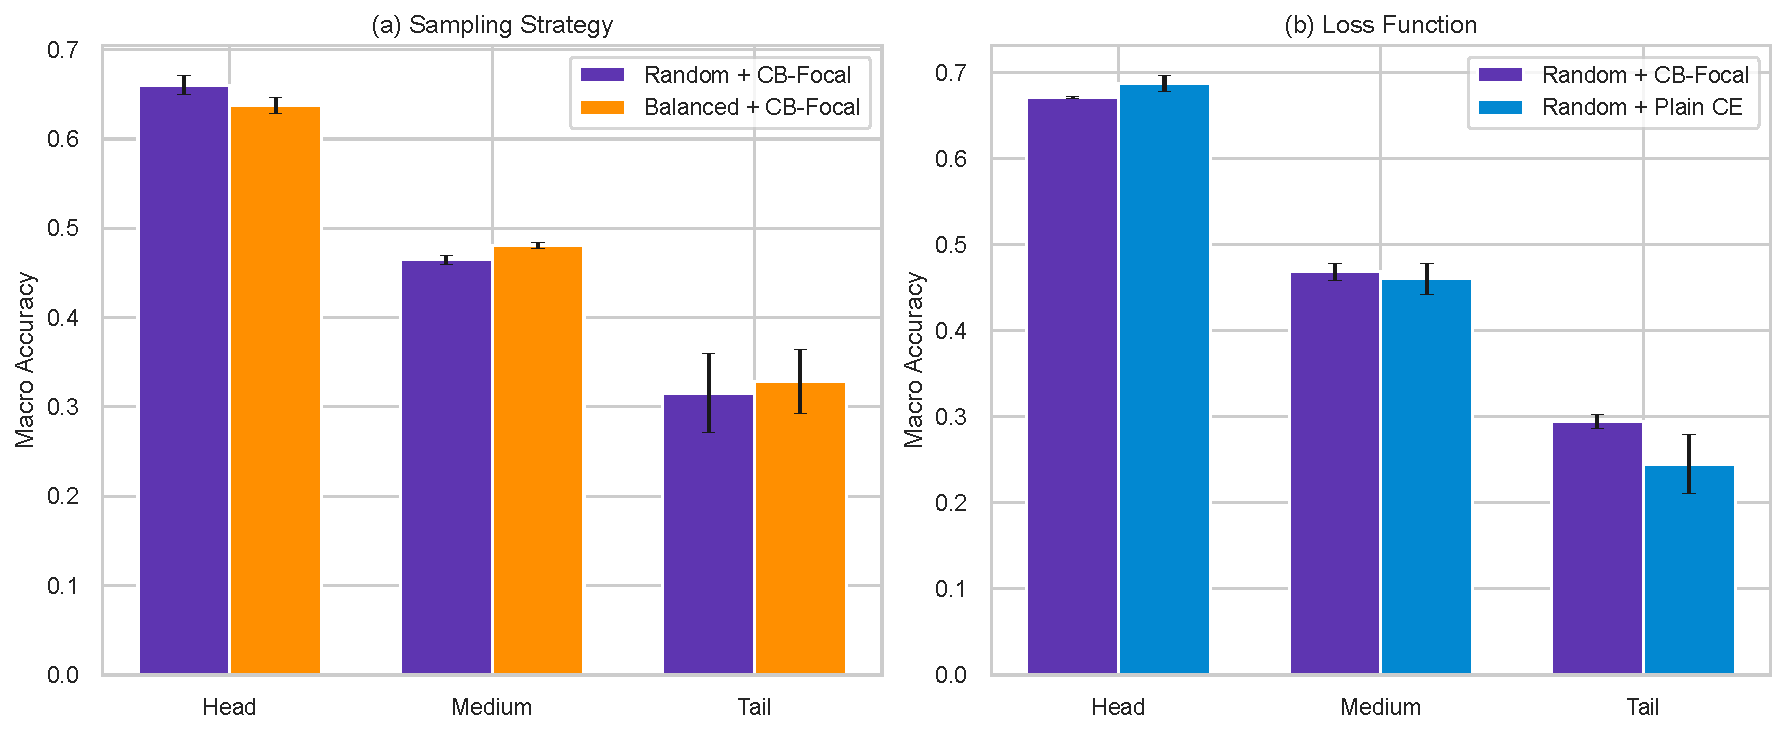
\includegraphics[width=\linewidth,keepaspectratio]{figure5.pdf}
\caption{Effect of long-tail training strategies on species-frequency groups under the same frozen DINOv3 configuration. Results are reported as mean ± standard deviation over three seeds. (a) Comparison between random and balanced sampling strategies. (b) Effect of applying Class-Balanced Focal Loss (CB-Focal) compared to Plain Cross-Entropy (Plain CE).}
\label{fig:figure5}
\end{figure}

Figure~\ref{fig:figure5}(b) shows the effect of using different loss functions, comparing Plain
Cross-Entropy (Plain CE) against Class-Balanced Focal Loss (CB-Focal)
\citep{ref14,ref63}
. As shown, CB-Focal loss gives significant increase in the rare
species, increasing the tail Macro Accuracy from 0.245 ± 0.034 to 0.294
± 0.008. Although the head class performance is slightly decreased, from
0.687 ± 0.009 to 0.671 ± 0.001, the significant gain on the long tail is
highly advantageous. The results indicate that even though balanced
sampling failed to achieve enough improvement to validate its cost on
frequent classes, integrating CB-Focal loss when the backbone capacity
is restricted could lessen the dataset's long tail issue.

\subsection{Qualitative Analysis}\label{qualitative-analysis}

By examining both the representative prediction of the Proposed Model
and the attention pattern obtained from its multi-context architecture,
this qualitative analysis was made. Figure~\ref{fig:figure6} reports two representative
test samples: a correctly classified \emph{Lethrinus punctulatus}
example and a misclassified Caranx ignobilis example predicted as
Gnathanodon speciosus. Where the figure also shows the MCEAM
cross-attention maps related to social, habitat, and full-frame context
streams, as well as backbone attention rollout for the ROI for each
sample.

The misclassified sample illustrates that contextual information does
not necessarily result in accurate species classification under visually
challenging conditions. In addition, the attention patterns include the
surrounding environment regions along side the target fish, indicating
the different visual information which the multi-context representation
includes. On the other hand, the correctly classified demonstrates how
the model's ability to adapt to various spatial regions surrounding the
target fish by using the model's contextual streams.



\begin{figure}[H]
\centering
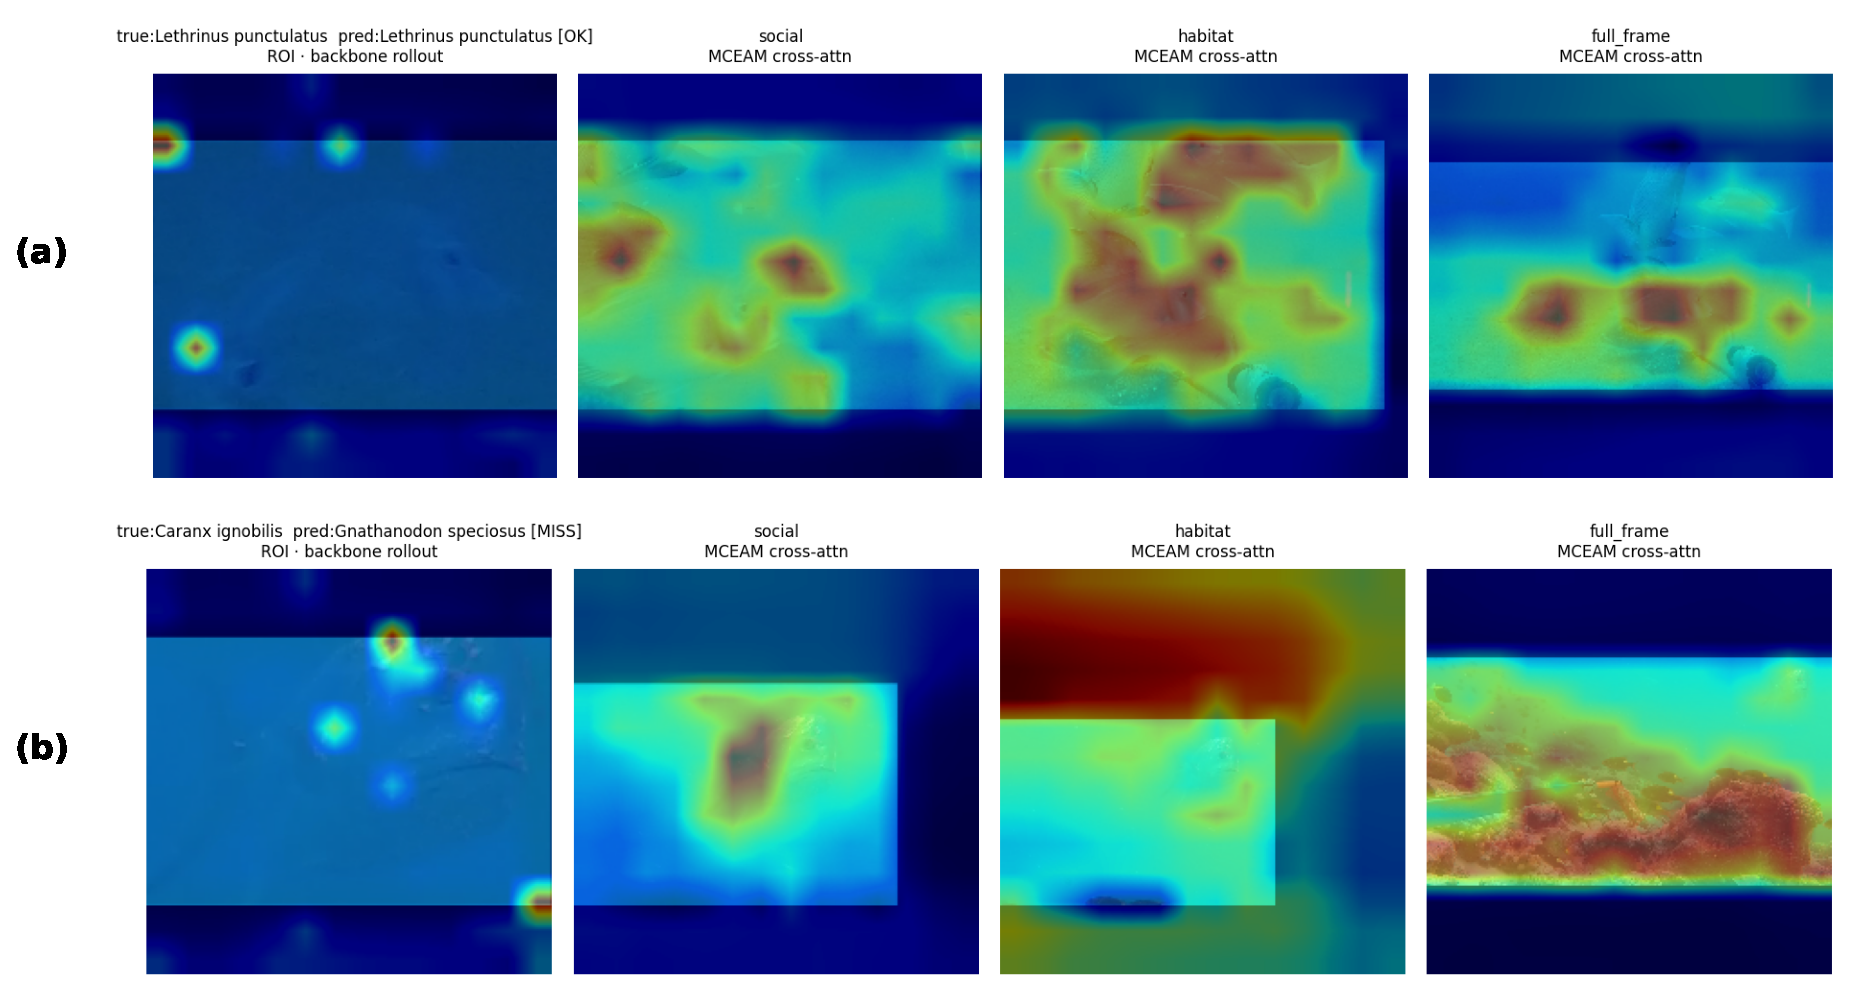
\includegraphics[width=\linewidth,keepaspectratio]{figure6.pdf}
\caption{Qualitative predictions and multi-context attention visualizations from the Proposed Model. (a) Correct classification of Lethrinus punctulatus. (b) Misclassification of Caranx ignobilis as Gnathanodon speciosus.}
\label{fig:figure6}
\end{figure}

These
visualization shows how the Proposed Model distributes attention across
the target in addition to its surroundings. They are intended to
complement the quantitative context and classification analyses rather
than serve as causal explanations of the model\textquotesingle s
predictions.

\subsection{Computational
Efficiency}\label{computational-efficiency}

\footnotesize\setlength{\tabcolsep}{3pt}
\begin{longtable}[]{@{}
  >{\raggedright\arraybackslash}p{(\columnwidth - 6\tabcolsep) * \real{0.2592}}
  >{\raggedright\arraybackslash}p{(\columnwidth - 6\tabcolsep) * \real{0.2469}}
  >{\raggedright\arraybackslash}p{(\columnwidth - 6\tabcolsep) * \real{0.2469}}
  >{\raggedright\arraybackslash}p{(\columnwidth - 6\tabcolsep) * \real{0.2469}}@{}}
\caption{Model size and predictive performance on the OzFish benchmark: total parameter count, Macro Accuracy, and Mean Hierarchical Distance (MHD).}\\
\toprule\noalign{}
\begin{minipage}[b]{\linewidth}\raggedright
Model
\end{minipage} & \begin{minipage}[b]{\linewidth}\raggedright
Total Parameters
\end{minipage} & \begin{minipage}[b]{\linewidth}\raggedright
Macro Accuracy
\end{minipage} & \begin{minipage}[b]{\linewidth}\raggedright
MHD
\end{minipage} \\
\midrule\noalign{}
\endhead
\bottomrule\noalign{}
\endlastfoot
Linear Probe & 85,907,265 & 0.471 ± 0.002 & 0.764 ± 0.003 \\
ResNet-50 & 24,165,761 & 0.571 ± 0.007 & 0.539 ± 0.005 \\
EfficientNetV2-S & 20,588,689 & 0.624 ± 0.013 & 0.447 ± 0.010 \\
ConvNeXt-T & 28,066,977 & 0.662 ± 0.002 & 0.373 ± 0.004 \\
ViT-B & 86,045,505 & 0.658 ± 0.010 & 0.377 ± 0.011 \\
Swin-B & 87,072,249 & 0.689 ± 0.009 & 0.347 ± 0.008 \\
MATANet & 1,347,468,072 & 0.692 ± 0.012 & 0.288 ± 0.008 \\
Proposed Model & 98,157,378 & 0.690 ± 0.023 & 0.291 ± 0.008 \\
\end{longtable}
\makeatletter
\edef\@currentlabel{\thetable}
\def\@currentlabelname{Model size and predictive performance on the OzFish benchmark: total parameter count, Macro Accuracy, and Mean Hierarchical Distance (MHD).}
\makeatother
\label{tab:computational-efficiency}
\normalsize\setlength{\tabcolsep}{6pt}

Table~\ref{tab:computational-efficiency} reports the computational performance of the evaluated models.
MATANet \citep{ref26} contains 1,347,468,072
parameters, where on the other hand, the Proposed Model contains
98,157,378 parameters, equivalent to approximately one-fourteenth of the
total number of parameters. Even though the huge difference in model
size, their benchmarking performance is still almost the same, with
MATANet achieving a Macro Accuracy of 0.692 ± 0.012 and a MHD of 0.288 ±
0.008, compared with 0.690 ± 0.023 and 0.291 ± 0.008, respectively, for
the Proposed Model.

Another model that is worth referencing is Swin-B
\citep{ref38}, which provides a parameter count
similar to the Proposed Model, equal to 87,072,249 parameters. It
achieves a Macro Accuracy of 0.689 ± 0.009 and a MHD of 0.347 ± 0.008,
showing similar overall classification accuracy but a higher
hierarchical error than the Proposed Model.

The results show that the Proposed Model was able to perform comparable
to MATANet while using approximately 7.3\% of its total parameters,
emphasizing a huge different balance between classification performance
and model scale.

\subsection{Overall Findings}\label{overall-findings}

The decisions made in order to reach the final Proposed model came from
the benchmark and ablation experiments. Among the architectural changes
that were assessed, the one with the largest improvement was the
backbone adaptation, progressively greater fine-tuning of the DINOv3
backbone resulted in an increase in Macro Accuracy and decrease in MHD.
Additionally, the ablation studies indicated that contextual information
also provides significant improvements over ROI-only classification, on
the other hand, increasing the attention depth over the initial settings
did not result in constant benefits.

A different type of improvement was observed in the taxonomy-aware
objective ablation. Even though Top-1 species level accuracy remained
almost similar to the flat objective, however, integrating the taxonomy
hierarchy decreased both metrics, MHD and MMS, while increasing genus
and family level accuracy. Since hierarchical
supervision\textquotesingle s primary contribution was to improve
taxonomic consistency rather than simply an increase in exact species
accuracy \citep{ref24}, this influenced the
decision to include it in the final model.

The ablation that further affected the selection of the final strategy
was long-tail experiments. Using the frozen DINOv3 as the main setting,
CB-focal \citep{ref14,ref63} resulted in better performance in
the tail-group than plain cross-entropy while both use random sampling,
showing that when the backbone remains restricted, using explicit
class-imbalance handling is beneficial. However, the final Proposed
Model uses a fully fine-tunned DINOv3 backbone, therefore, using plain
cross entropy and random sampling achieved significantly better tail
results than the frozen configuration. The results suggest that the
long-tail strategy performance depends on the representation-learning
approach \citep{ref10,ref65}. Under constrained frozen backbone
training, CB-focal displays noticeable improvements, on the other hand,
using the full adapted model perform better without requiring an
additional loss modification.

As a result, the final model configuration combined the parts that
consistently contributed to the ablation study: task-specific backbone
adaptation, multi-context representation, taxonomy-aware supervision,
and a simpler plain cross-entropy objective. The Proposed Model achieves
0.690 ± 0.023 Macro Accuracy and 0.291 ± 0.008 MHD on the benchmark,
while keeping performance equivalent to MATANet at a significantly
smaller model scale.

\section{Limitations}\label{limitations}

Due to the nature of this work, there were certain limitations that we
faced during the benchmark, specifically within the curated Ozfish
benchmark itself. The main limitation that had to be considered was the
fact that the dataset has a long-tail distribution, and even though
there were measures taken to mitigate class imbalance, the results still
showed that the models often underperformed with tail species due to
their small sample sizes. The deployment-aware split also introduces
limitations for the rarest species. Since some species are represented
by a small number of observations or deployments, they cannot always be
represented across all dataset partitions, which may reduce the
stability of validation and test estimates for low-frequency classes,
although maintaining deployment independence is important to avoid
overly optimistic performance caused by highly related samples appearing
in multiple folds \citep{ref17,ref20}.

Another important limitation to discuss is the geographic specificity of
the benchmark. All the experiments that the models were evaluated under
were based on the species and ecology of the Australian marine
ecosystems represented in the curated OzFish benchmark, meaning that
they may not generalize well in a different region, as each region
differs in its ecological distribution as well as environmental
conditions \citep{ref13,ref18}. Evaluation on independent datasets
from other marine regions would be necessary to assess model
generalization across different environments beyond OzFish.

The taxonomy-aware evaluation also provides a simplified representation
of error severity. Hierarchical errors are categorized according to
species, genus, and family membership, allowing taxonomically closer and
more distant mistakes to be distinguished consistently. This ordinal
measure, however, does not represent continuous phylogenetic or
ecological distance between species.

Lastly, the ablation analysis also has a limitation in that several
architectural ablations, including the context and MCEAM-depth
comparisons, were conducted under a frozen DINOv3 configuration, whereas
the final proposed model uses full backbone fine-tuning. These
experiments therefore isolate the corresponding architectural choices
within their matched experimental setting, but do not fully characterize
possible interactions between contextual fusion and backbone adaptation.

\section{Conclusion and future
work}\label{conclusion-and-future-work}

This paper introduced a fine-grained species classification benchmark
built on the OzFish dataset, together with a taxonomy-aware
multi-context classifier evaluated on it. OzFish combines survey-grade
BRUVS imagery with family, genus, and species annotations, but it has
been released without a standard classification split, so published
results on it are neither directly comparable nor protected against
leakage between the highly correlated frames that a single deployment
produces. The benchmark addresses this by curating the dataset to 76,083
crops spanning 321 species, and by partitioning it at the level of the
BRUVS deployment rather than the individual crop, so that stereo pairs
and near-duplicate frames of the same individual cannot fall on both
sides of the train and test boundary. The resulting split is released so
that later work can be evaluated on identical data. The proposed model
encodes the target fish alongside three progressively wider views of its
surroundings, fuses them through cross-attention under a learned gate
that weighs contextual evidence against target morphology, and obtains
genus- and family-level probabilities by marginalising a single species
distribution, which keeps predictions consistent across taxonomic levels
by construction.

Eight models spanning convolutional, transformer, self-supervised, and
context-aware families were evaluated over three seeds under a common
protocol, using a metric panel that combines conventional accuracy with
taxonomy-aware and frequency-stratified measures. Performance rose
steadily with backbone capability across the conventional baselines,
from a macro accuracy of 0.571 for ResNet-50 to 0.689 for Swin-B,
indicating that the benchmark remains difficult enough to separate
representations of differing strength. The proposed model reached a
macro accuracy of 0.690 and a Top-1 accuracy of 0.842, with an MHD of
0.291 and a family-level accuracy of 0.951, achieving mean performance
comparable to MATANet across the headline metrics while using a
considerably smaller backbone. The metric panel also proved necessary
rather than decorative, since models with comparable Top-1 accuracy
differed measurably in the taxonomic severity of their errors. Accuracy
fell consistently as species frequency decreased, and tail performance
was consistently the weakest and generally more variable across seeds,
which remains the principal limitation of the benchmark alongside its
restriction to Australian marine ecosystems.

Three directions follow from these results. The clearest remaining
headroom lies in the tail, where reweighting alone proved insufficient
and where methods that adjust the classifier rather than the loss, such
as logit adjustment or decoupled classifier retraining
\citep{ref65}, are worth testing on this
benchmark. A second direction is temporal, as BRUVS footage provides
short clips around each annotated frame, and aggregating predictions
over a sequence rather than a single view may recover species that one
degraded frame cannot resolve \citep{ref50}.
Finally, applying the benchmark protocol to survey data from other
marine regions \citep{ref13} would establish
whether the deployment-grouped design and the observed ranking of
methods hold beyond Australian waters. By releasing the split, the
protocol, and the baseline results, this work aims to give subsequent
studies of fine-grained marine recognition a common and
leakage-controlled basis for comparison.

\section*{Declaration of generative AI and AI-assisted technologies in the manuscript preparation process}

During the preparation of this work, the authors used ChatGPT to assist
with manuscript organization, language and presentation, LaTeX
preparation, reference and consistency checks, and review against
journal submission requirements. The authors reviewed and verified the
resulting assistance, edited the manuscript as needed, and take full
responsibility for the content of the publication.

\section*{Declaration of competing interest}

The authors declare that they have no known competing financial
interests or personal relationships that could have influenced the work
reported in this paper.

\section*{Data and code availability}

The original OzFish dataset used in this study is publicly available
from the Australian Institute of Marine Science at
\url{https://doi.org/10.25845/5e28f062c5097}. The benchmark code and split repository link is withheld for double-anonymized review.

\bibliographystyle{elsarticle-harv}
\bibliography{references}

\end{document}
